% ============================================================
% IMAGE RENAME GUIDE (rename your screenshots as below and
% place them in the same folder as this .tex file):
%
%  --- SESSION 1 (2026-04-21) ---
%  ipconfig_lab.jpg        lab machine ipconfig
%  ipconfig_mridul.jpg     scanning host ipconfig (session 1)
%  netA_scan.jpg           Network A scan
%  netA_cve.jpg            Network A CVE
%  netB_full.jpg           Network B full view
%  netB_cve.jpg            Network B CVE
%  netB_whatif.jpg         Network B what-if
%  netC_full.jpg           Network C full view
%  netC_chains.jpg         Network C chains
%  netC_mitre.jpg          Network C MITRE
%  netC_cve.jpg            Network C CVE
%  netC_whatif.jpg         Network C what-if
%
%  --- SESSION 2 (2026-04-23) ---
%  netE_chains1.jpg        Network E chains page 1
%  netE_chains2.jpg        Network E chains page 2
%  netE_critical1.jpg      Network E critical paths 1
%  netE_critical2.jpg      Network E critical paths 2
%  netE_critical3.jpg      Network E critical paths 3
%  netE_mitre.jpg          Network E MITRE ATT&CK
%  netE_scan.jpg           Network E scan results
%  netF_dashboard.jpg      Network F dashboard
%  netF_full.jpg           Network F full attack graph
%  netF_critical1.jpg      Network F critical paths
%  netF_mitre.jpg          Network F MITRE ATT&CK
%  netF_chains.jpg         Network F attack chains
%  netF_cve.jpg            Network F CVE database
%  netF_whatif.jpg         Network F what-if analysis
%  netG_dashboard.jpg      Network G dashboard (172.20.10.3)
%  netG_dashboard2.jpg     Network G attack graph + scan results
%  netH_dashboard.jpg      Network H dashboard (8.8.8.8)
%  netH_chains.jpg         Network H attack chains
%  netH_critical.jpg       Network H critical paths 1
%  netH_critical2.jpg      Network H critical paths 2
%  netH_critical3.jpg      Network H critical paths 3
%  netH_mitre.jpg          Network H MITRE ATT&CK
%  ipconfig_mridul2.jpg    scanning host ipconfig (session 2)
%
%  --- SESSION 3 (2026-05-03) ---
%  netA_dashboard.jpg      Network A clean dashboard (NES=0)
%  netC_whatif_smb.jpg     Network C What-If: SMB/RPC
%  netC_whatif_netbios.jpg Network C What-If: NetBIOS/SMB
%  ipconfig_mridul3.jpg    scanning host ipconfig (session 3)
%  (ipconfig_lab.jpg)      lab machine ipconfig (reused from session 1)
% ============================================================

\documentclass[conference]{IEEEtran}
\IEEEoverridecommandlockouts
\usepackage{cite}
\usepackage{amsmath,amssymb,amsfonts}
\usepackage{algorithmic}
\usepackage{graphicx}
\graphicspath{{figures/}}
\usepackage{subcaption}
\usepackage{textcomp}
\usepackage{xcolor}
\usepackage{booktabs}
\usepackage{multirow}
\def\BibTeX{{\rm B\kern-.05em{\sc i\kern-.025em b}\kern-.08em
    T\kern-.1667em\lower.7ex\hbox{E}\kern-.125emX}}

\begin{document}

\title{NET\_SCAN: Automated Lateral Movement Detection \& Cyber Kill Chain Modeling
\thanks{This research outlines the architectural design and experimental validation of the NET\_SCAN platform across eight heterogeneous network environments.}
}

\author{\IEEEauthorblockN{Mridul Singh Rawat}
\IEEEauthorblockA{\textit{School of Computer Science} \\
\textit{University of Petroleum and Energy Studies (UPES)}\\
Dehradun, India \\
Mridul.119881@stu.upes.ac.in}
\and
\IEEEauthorblockN{Akshat Joshi}
\IEEEauthorblockA{\textit{School of Computer Science} \\
\textit{University of Petroleum and Energy Studies (UPES)}\\
Dehradun, India \\
Akshat.125233@stu.upes.ac.in}
\and
\IEEEauthorblockN{Gagan Deep Singh}
\IEEEauthorblockA{\textit{School of Computer Science} \\
\textit{University of Petroleum and Energy Studies (UPES)}\\
Dehradun, India \\
gagan.ddn@upes.ac.in}
}

\maketitle

\begin{abstract}
The network security scan reports we get now are long and hard to understand. They list all the vulnerabilities one by one which makes it tough for the person in charge to see how vulnerable the network is to cyber attacks. NET\_SCAN is a tool that scans the network in time and does more than just checking the ports. It shows us how an attacker can use vulnerabilities to move around the network. NET\_SCAN maps an attack path, like a diagram that shows how the attacker can get in through the open ports and move through its target through the shortest path. The tool uses technique called the Cyber Kill Chain framework and MITRE ATT\&CK mappings to make this map. It also uses algorithms, like the BFS algorithm which finds the shortest way the attacker can get in and Dijkstras algorithm to find the most damaging way. The program also figures out how risky the network is overall using the Network Exposure Score. We tested NET\_SCAN on different network setups like a campus Wi-Fi network, some virtual machines and a few internet hosts that anyone can access. We even tested it on a file server and a public DNS resolver like 8.8.8.8. The tool worked well. Was able to identify the different parts of the network like the entry points the pivot points and the targets as well. It also collected information about the vulnerabilities from the National Vulnerability Database. Matched them with the right MITRE ATT\&CK tactics. This gave us an idea of how exposed the network is. NET SCAN is a useful tool, for network security.
\end{abstract}

\begin{IEEEkeywords}
Cyber Kill Chain, Lateral Movement, Attack Graphs, Network Security, MITRE ATT\&CK, Vulnerability Mapping, Network Exposure Score, BFS, Dijkstra
\end{IEEEkeywords}

% ============================================================
\section{Introduction}
% ============================================================
As the networks keep growing bigger and more connected securing them becomes difficult . The tools that we use every day like Nmap and Nessus are very good at finding weaknesses in single machines. But they don't clearly show how an attacker can connect these weaknesses together \cite{nmap_ref}, \cite{nessus_ref}. Now, just finding one weak machine is not enough. We need to understand the exact paths an attacker can take to move deeper into the network which is called lateral movement. Finding these attack paths manually takes a large amount of time and usually needs expert red team skills. To solve this problem, we created NET SCAN. It is an automated tool that simulates and maps attacks. It takes basic port scan data looks for vulnerabilities using the National Vulnerability Database (NVD) \cite{nvd_ref} and uses our custom algorithms to draw possible kill chains on an interactive graph. By converting simple text data into a visual graph, it becomes much easier to understand how far an attack can spread and which systems should be fixed first, using our Network Exposure Score (NES).

The main things that we achieved in this work are:
\begin{itemize}
    \item We built a fully automated pipeline that connects TCP port scanning, CVE lookups, and kill-chain mapping all into one browser interface.
    \item We created a critical path engine that runs on both BFS and Dijkstra algorithms to find and rank lateral movement paths based on risk.
    \item We developed a method to automatically predict pivot paths by mapping MITRE ATT\&CK techniques to the discovered services.
    \item We designed the Network Exposure Score (NES) it is a math-based formula that gives a network risk score from 0 to 100.
    \item We tested the tool on eight different networks, including local setups and real internet hosts like a public DNS resolver, to prove it works.
    \item We added a ``What-If'' feature that will allow you to simulate how to fix a vulnerability and instantly see how much it improves the NES score.
\end{itemize}

% ============================================================
\section{Related Work}
% ============================================================
A lot of research has already been done on attack graphs \cite{ammann2002}. For example: BloodHound \cite{bloodhound} changed the way we secure Active Directory (AD) by using graphs to find out hidden paths attackers use to gain higher privileges. However, the limitation of BloodHound is that it only focuses on AD environments.

With NET SCAN, our aim was to bring the same visual approach to normal TCP/IP networks. Instead of giving just a static report, NET SCAN calculates the current strength of the network and shows the graph live in the browser. What makes NET SCAN different is its Critical Paths engine. We run both BFS and Dijkstra algorithms together this helps us see both the shortest path an attacker can take and the most dangerous one at the same time.

% ============================================================
\section{System Architecture}
% ============================================================
We split the tool into two main parts: a Python backend that handles the heavy lifting like scanning and intelligence gathering, and a frontend built with React and HTML5 Canvas to draw the graphs.

\subsection{Heuristic Kill Chain Classification}
When NET\_SCAN finds an open service, it automatically tries to figure out what role it plays in an attack. We break them down into three categories:
\begin{itemize}
    \item \textbf{Entry Nodes:} Things like web servers (ports 80, 443) or FTP that are exposed to the outside and give an attacker their first foothold.
    \item \textbf{Pivot Nodes:} The services like SSH or RDP that an attacker could use to hop into deeper and more restricted parts of the network.
    \item \textbf{Target Nodes:} The final goal of the attack, like a DNS server or a Domain Controller holding sensitive data.
\end{itemize}

\subsection{Automated Lateral Movement Modeling}
NET\_SCAN guesses how these nodes connect (like going from $Entry \rightarrow Pivot \rightarrow Target$) by looking at MITRE techniques. For example: it checks for techniques like Exfiltration Over Alt Protocol (T1048) or Exploiting Remote Services (T1210). To decide if a path is usable by a hacker it checks the live CVE data that it pulls from the NVD.

\subsection{Critical Paths Engine}
Our Critical Paths Engine is unique because it can run two graph algorithms at the same time:
\begin{itemize}
    \item \textbf{BFS (Shortest Path):} This find out the quickest way to a target node counting the fewest number of jumps.
    \item \textbf{Dijkstra (Deadliest Path):} This looks at the CVSS severity scores of the vulnerabilities. It finds the path that has the most critical flaws, which we label as \textsc{deadliest} in the app.
\end{itemize}
Every path gets a hop count and a Risk score so you know exactly which paths are the most dangerous.

\subsection{Network Exposure Score (NES)}
To give the network a simple grade, we created the NES. It combines the CVSS 3.1 scores of the vulnerabilities with the number of possible attack paths.
Here is the math behind the NES ($S_{exp}$):
\begin{equation}
S_{exp} = \sum_{i=1}^{N} (w_{cve}^{(i)} \times D_{node}^{(i)}) \times \alpha^{P}
\end{equation}
In this formula, $w_{cve}^{(i)}$ is how severe the vulnerability is, $D$ is the depth, $P$ is the number of lateral paths, and $\alpha$ is a multiplier for the blast radius. We scale the result from 0 to 100 and group it into four tiers: Low (0--30), Medium (31--59), High (60--80) and Critical (81+).

\subsection{What-If Mitigation Engine}
We built a ``What-If'' feature so that you can play around with the graph. You can click on a vulnerable service and simulate taking it offline. When you do this, NET SCAN recalculates the NES and the attack chains instantly. This let you see exactly how safer your network would be if you patched a specific bug. We tested this heavily on Networks C and F and found it perfectly tracked how much the risk dropped when we disabled certain ports.

% ============================================================
\section{Experimental Validation}
% ============================================================
To prove that our mapping engine, CVE lookups, and exposure scoring actually work in the real world, we tested NET SCAN on eight different networks. We chose the environments that varied wildly how they were set up and what services they ran.

\subsection{Testing Environment}
We ran our tests against eight network segments that we could reach from our scanning laptop. Each one represented a totally different type of network. You can see our exact network adapter setups during these test sessions in Figs.~\ref{fig:ipconfig}, \ref{fig:ipconfig2}, and \ref{fig:ipconfig3}.

\begin{figure}[htbp]
\centerline{
  \begin{subfigure}[b]{0.48\linewidth}
    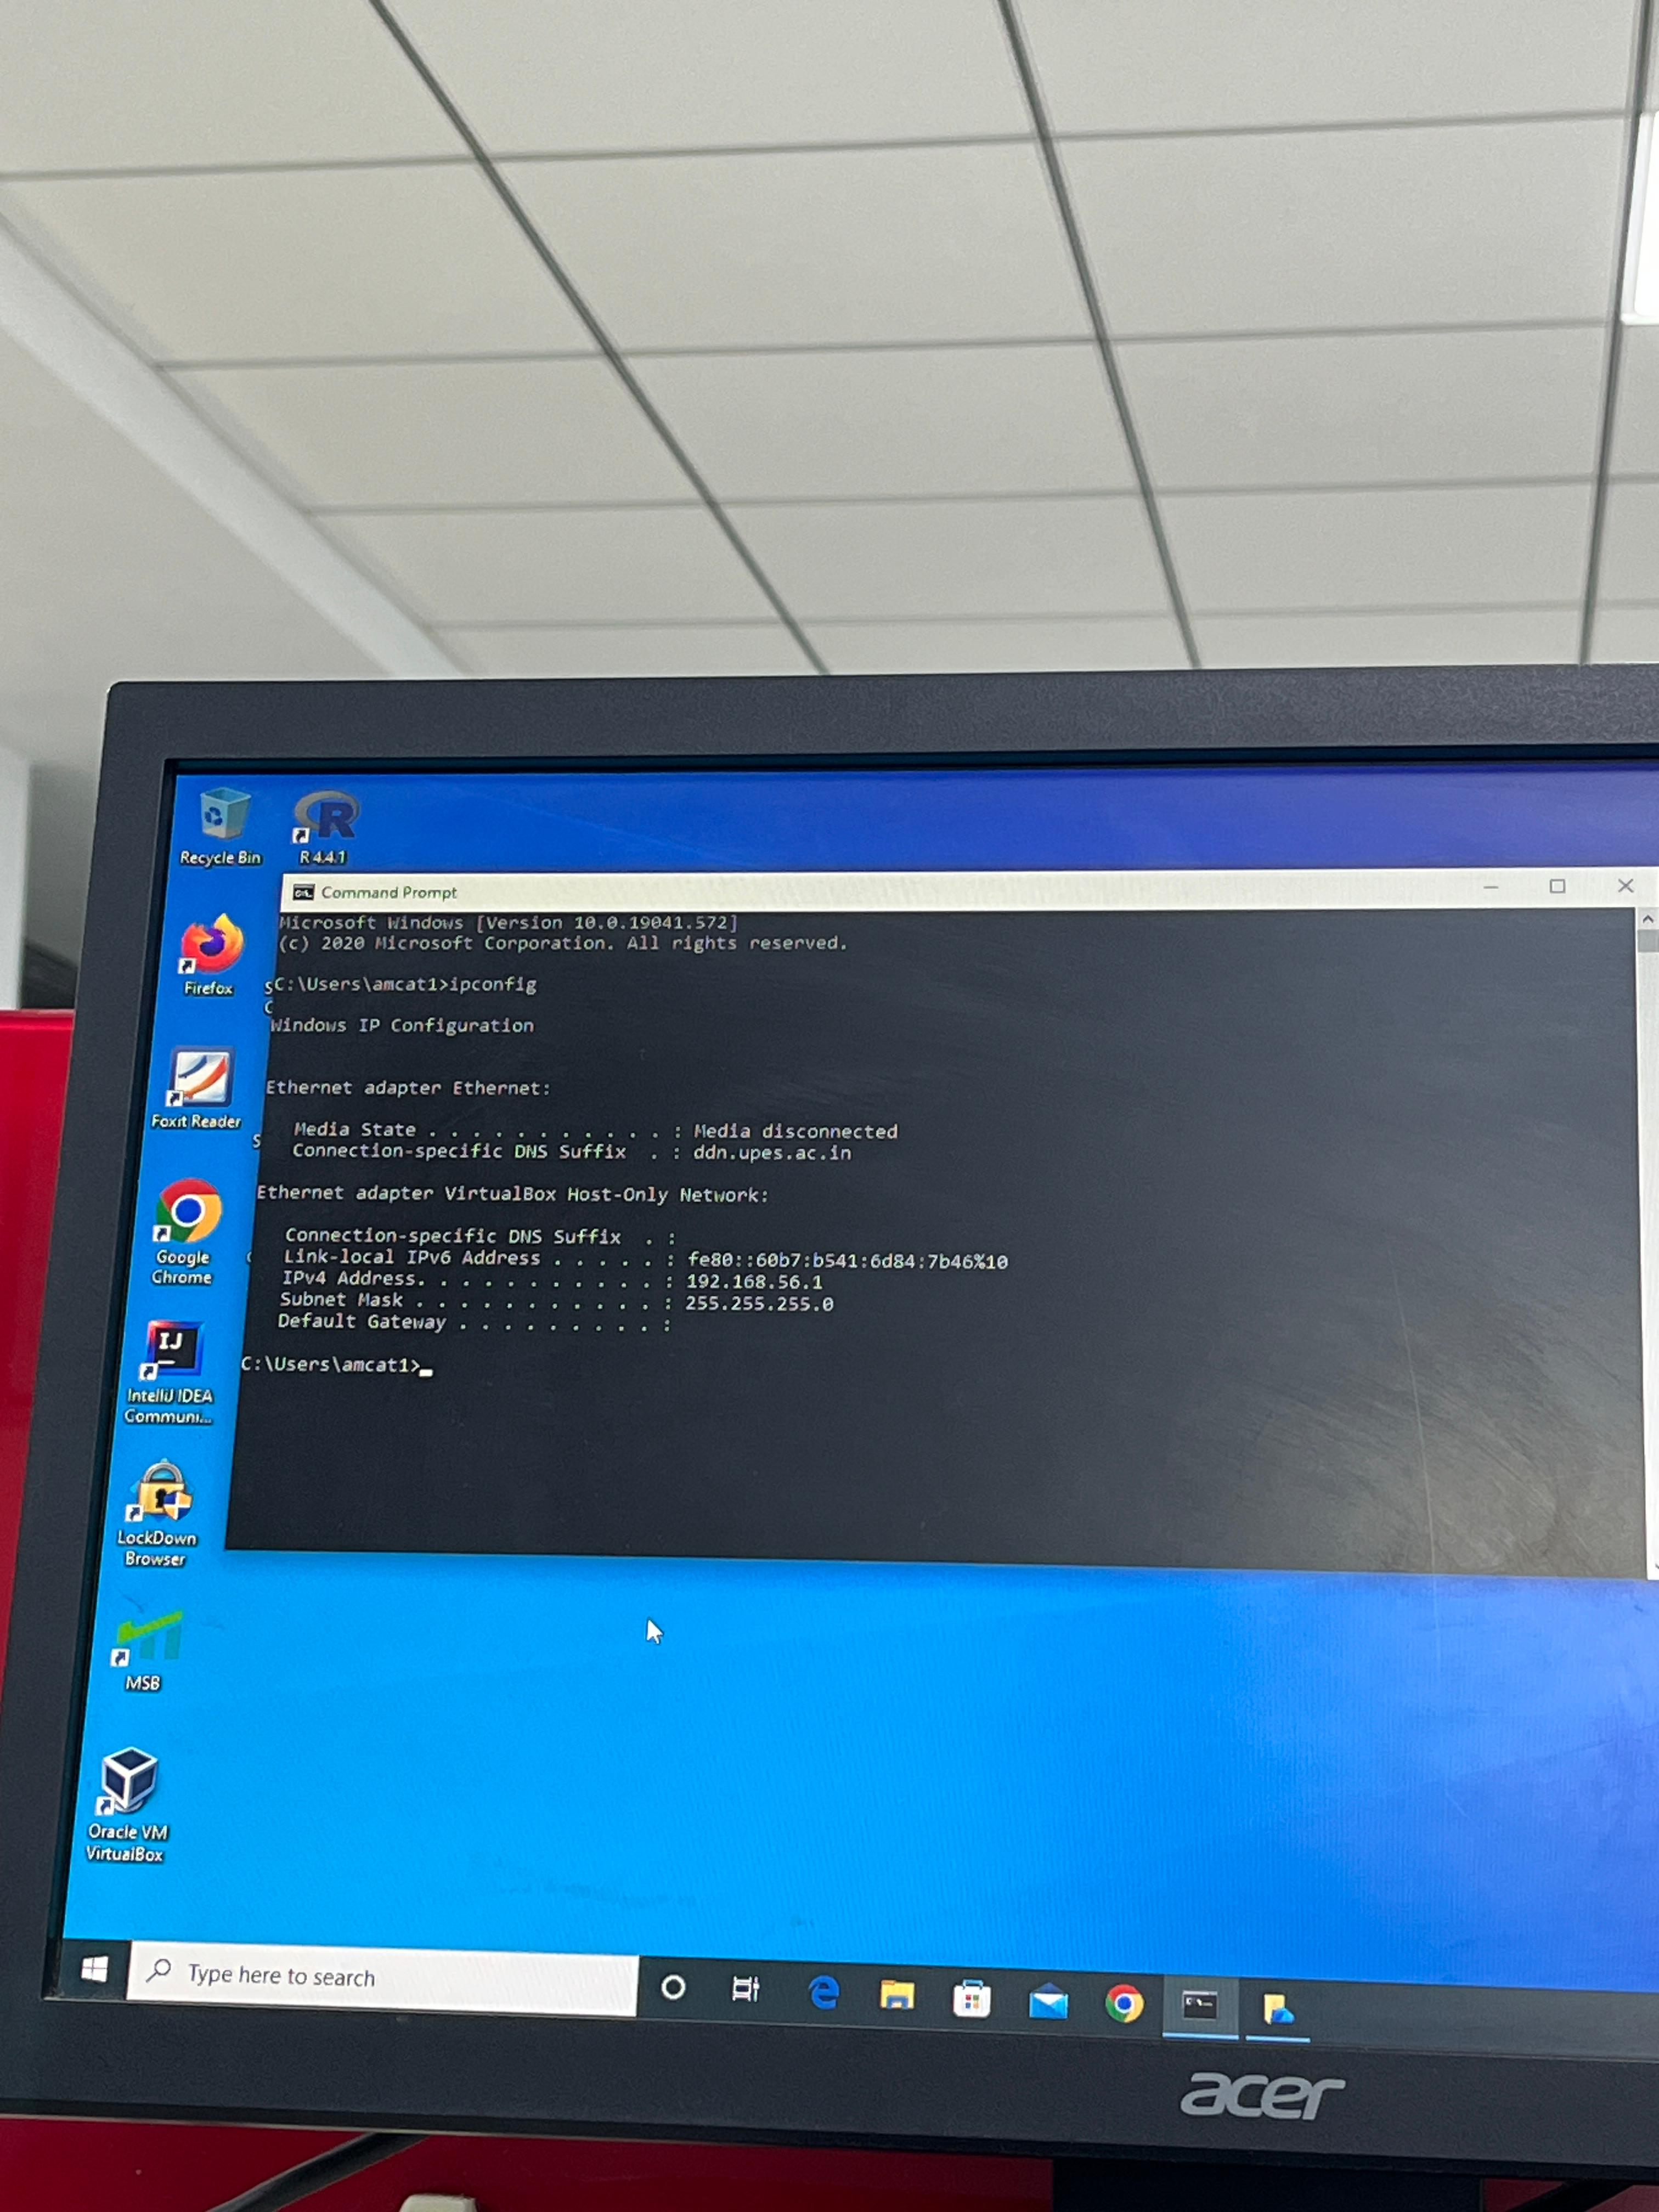
\includegraphics[width=\linewidth]{ipconfig_lab.jpg}
    \caption{Lab machine \texttt{ipconfig}: VirtualBox adapter at 192.168.56.1, Wi-Fi at 10.68.124.117.}
    \label{fig:ipconfig_lab}
  \end{subfigure}
  \hfill
  \begin{subfigure}[b]{0.48\linewidth}
    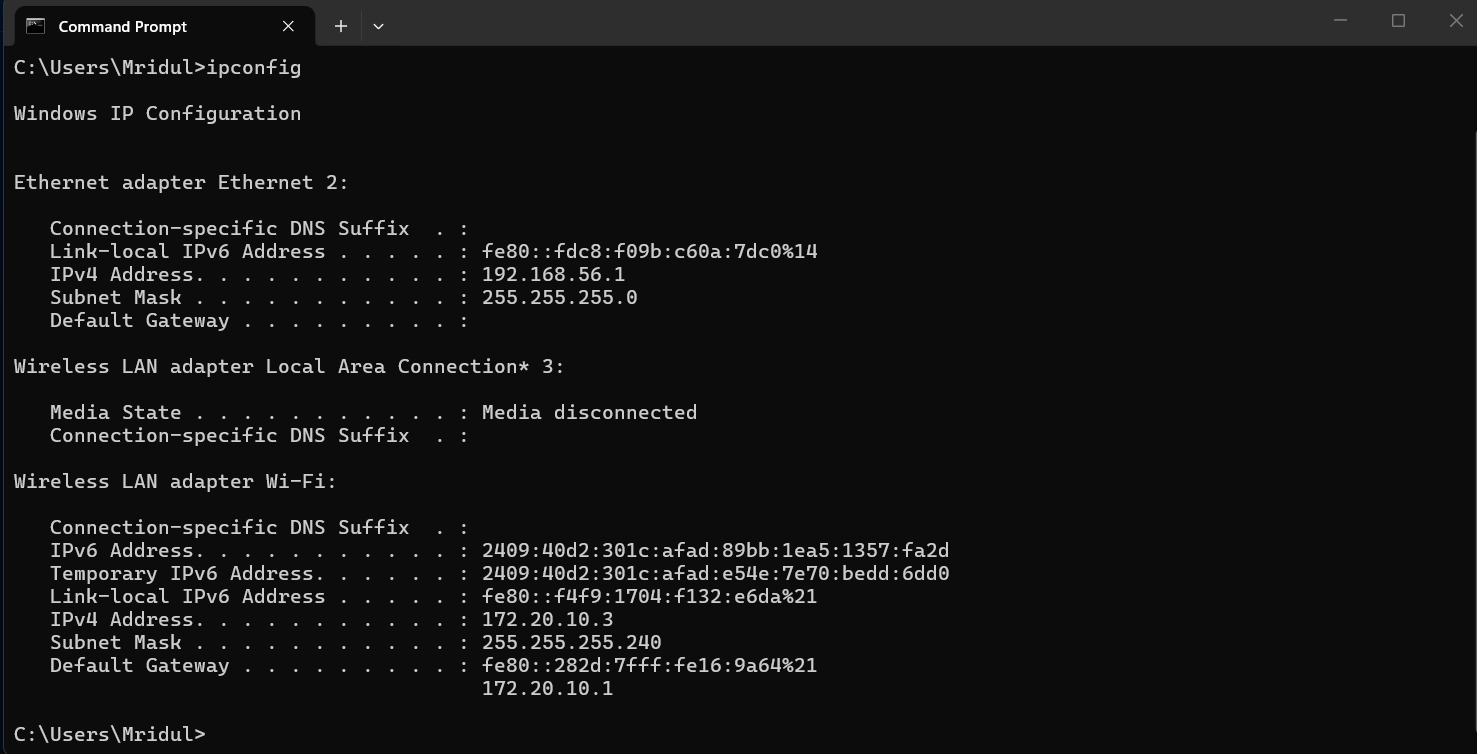
\includegraphics[width=\linewidth]{ipconfig_mridul.jpg}
    \caption{Scanning host \texttt{ipconfig} (session 1): VirtualBox adapter 192.168.56.1 and Wi-Fi 172.20.10.3.}
    \label{fig:ipconfig_mridul}
  \end{subfigure}
}
\caption{Host machine network adapter configurations (session 1) confirming active interfaces.}
\label{fig:ipconfig}
\end{figure}

\begin{figure}[htbp]
\centerline{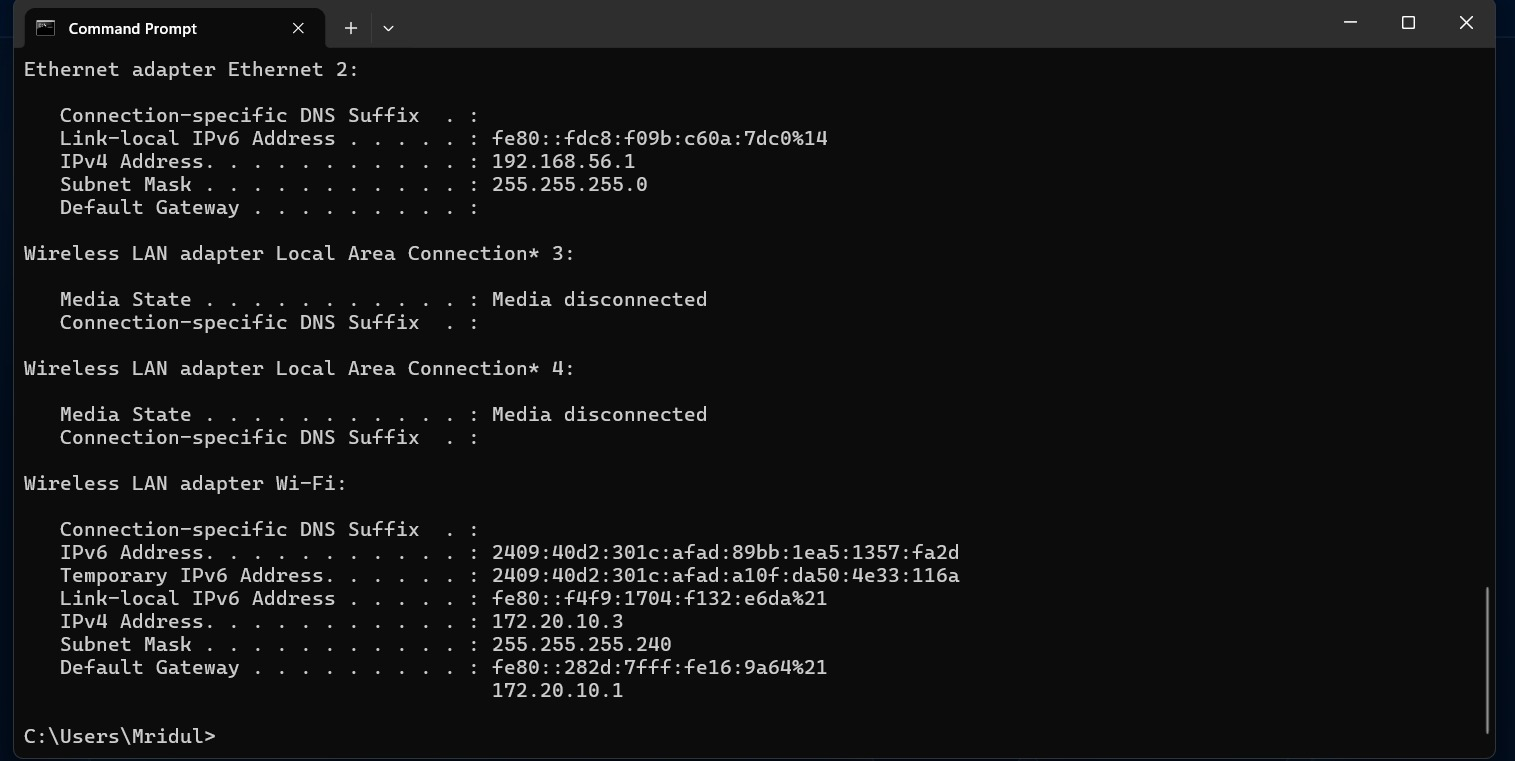
\includegraphics[width=0.75\linewidth]{ipconfig_mridul2.jpg}}
\caption{Scanning host \texttt{ipconfig} (session 2): Ethernet 2 adapter at 192.168.56.1; Wi-Fi adapter at 172.20.10.3 (subnet 255.255.255.240, gateway 172.20.10.1), confirming the active interfaces used for Networks G and H.}
\label{fig:ipconfig2}
\end{figure}

\begin{figure}[htbp]
\centerline{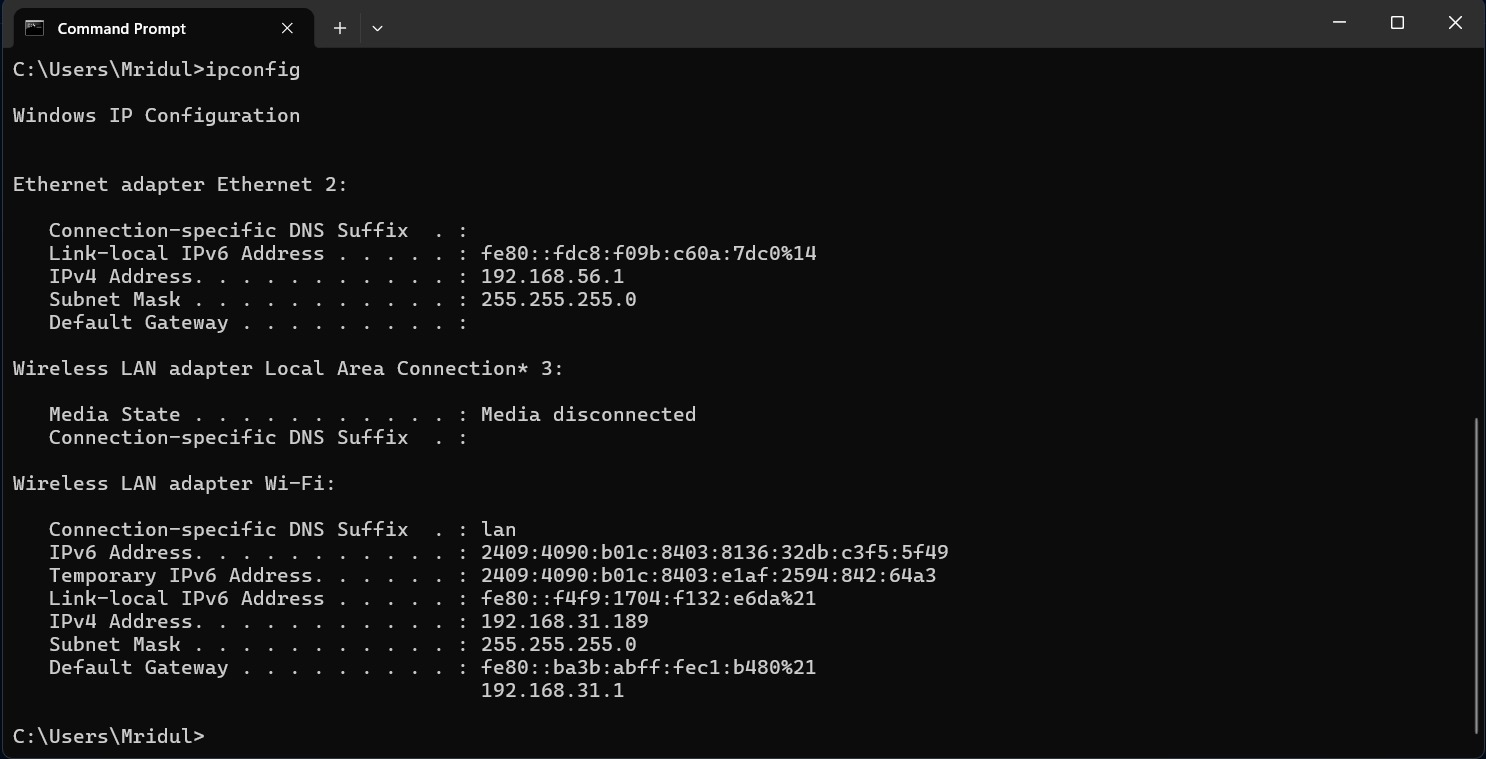
\includegraphics[width=0.75\linewidth]{ipconfig_mridul3.jpg}}
\caption{Scanning host \texttt{ipconfig} (session 3): Ethernet 2 adapter at 192.168.56.1 (VirtualBox Host-Only); Wi-Fi adapter at 192.168.31.189 (subnet 255.255.255.0, gateway 192.168.31.1), confirming the active interfaces used for the remediation validation session.}
\label{fig:ipconfig3}
\end{figure}

Here are the eight environments we tested:
\begin{itemize}
    \item \textbf{Network A (Campus Wi-Fi):} Target IP \texttt{10.68.124.5} --- Our own laptop connected to the university Wi-Fi.
    \item \textbf{Network B -- VirtualBox FTP Host:} Target IP \texttt{10.9.7.187} -- A virtual box running on the local computer using an old and vulnerable FTP server.
    \item \textbf{Network C -- VirtualBox Multi-Service:} Target IP \texttt{192.168.56.1} -- The VirtualBox host gateway running multiple services concurrently.
    \item \textbf{Network D -- Mobile Hotspot Bridge:} Target IP \texttt{192.168.137.1} -- A network created using a Windows mobile hotspot.
    \item \textbf{Network E -- Public Internet Host 1:} Target IP \texttt{208.67.222.222} -- The public server by OpenDNS. We found five open ports in it giving it a Critical NES value of 85.
    \item \textbf{Network F -- Public Internet Host 2:} Target IP \texttt{185.222.222.222} -- This network had the highest complexity. NES reached its maximum value of 100 here.
    \item \textbf{Network G -- Local SMB Host:} Target IP \texttt{172.20.10.3} -- Our own Wi-Fi adapter running Windows file sharing. It gave us NES 50, which is considered to be Medium.
    \item \textbf{Network H -- Google Public DNS:} Target IP \texttt{8.8.8.8} -- The world-famous DNS server by Google. Scanned to test the tool's effectiveness against a highly secure public server, it got NES 60.
\end{itemize}

\subsection{Scan Configuration}
We ran all these tests directly from our NET\_SCAN web dashboard using these settings:
\begin{itemize}
    \item \textbf{Port Range:} 1--1024 (the standard well-known ports).
    \item \textbf{Timeout:} 120--145\,ms per port.
    \item \textbf{Threads:} 1 (because we were testing one IP address at a time).
    \item \textbf{CVE Lookups:} Real-time lookups from the NVD API version 2.0.
    \item \textbf{Path Finding:} BFS/Dijkstra immediately after the scan.
\end{itemize}

\noindent\textit{Ethical Note:} When scanning public IPs (Networks E, F, H), we only used TCP SYNs to ports 1--1024 and did not engage in any exploitation or malicious activities.

% ============================================================
\subsection{Results \& Findings}
% ============================================================

\subsubsection{Aggregate Scan Metrics}
The following table summarizes the quantitative data collected during scans of all eight target network environments.

\begin{table}[htbp]
\caption{NET\_SCAN Experimental Validation Results Across Eight Network Environments}
\begin{center}
\begin{tabular}{|l|c|c|c|c|c|c|c|c|}
\hline
\textbf{Metric} & \textbf{A} & \textbf{B} & \textbf{C} & \textbf{D} & \textbf{E} & \textbf{F} & \textbf{G} & \textbf{H} \\
\hline
Open Ports & 0 & 1 & 3 & 0 & 5 & 7+ & 3 & 4 \\
\hline
CVEs & 0 & 3 & 6 & 0 & 6 & 6 & 6 & 6 \\
\hline
Critical Nodes & 0 & 1 & 2 & 0 & 2 & 2 & 2 & 1 \\
\hline
High Risk & 0 & 0 & 1 & 0 & 3 & 5 & 1 & 3 \\
\hline
Services & 0 & 1 & 3 & 0 & 5 & 7 & 3 & 4 \\
\hline
Lateral Paths & 0 & 0 & 0 & 0 & 3 & 7 & 0 & 2 \\
\hline
Connections & 0 & 0 & 3 & 0 & 3 & 9 & 3 & 3 \\
\hline
MITRE Tech. & 0 & 0 & 2 & 0 & 5 & 3 & 2 & 2 \\
\hline
\textbf{NES} & \textbf{0} & \textbf{20} & \textbf{50} & \textbf{0} & \textbf{85} & \textbf{100} & \textbf{50} & \textbf{60} \\
\hline
\textbf{Tier} & Low & Low & Med & Low & Crit & Crit & Med & High \\
\hline
\end{tabular}
\label{tab:scan_metrics}
\end{center}
\end{table}

% ============================================================
\subsubsection{Network A --- Campus Wi-Fi (10.68.124.5)}
% ============================================================
In the scanning of the network interface for the campus Wi-Fi, it was found that out of the 1024 TCP ports available, all were either closed or filtered, thereby generating no open ports at all. Therefore, the NES gave a perfect baseline value of 0, demonstrating the zero false-positive feature of the heuristic engine.

\begin{figure}[htbp]
\centerline{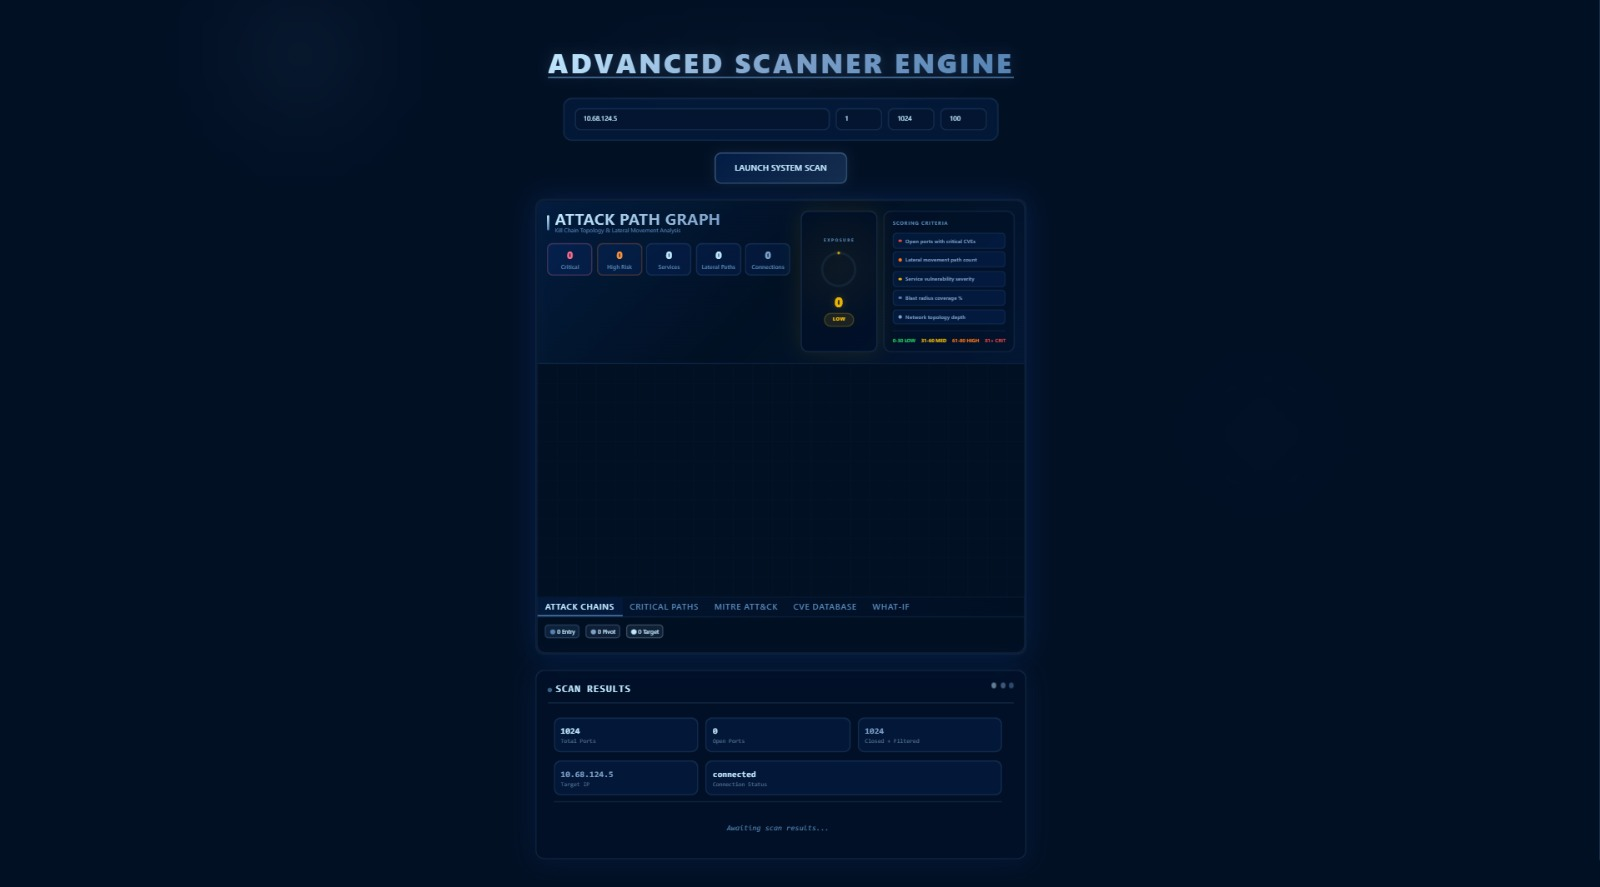
\includegraphics[width=0.95\linewidth]{netA_dashboard.jpg}}
\caption{NET\_SCAN dashboard for Network A (10.68.124.5): all metrics at zero---0 Critical, 0 High Risk, 0 Services, 0 Lateral Paths, 0 Connections---with NES = 0 (Low). The scan results pane confirms 1024 ports scanned, 0 open, and connection status ``connected''. This clean baseline validates the zero false-positive bound of the heuristic engine.}
\label{fig:netA_dashboard}
\end{figure}

% ============================================================
\subsubsection{Network B --- VirtualBox FTP Host (10.9.7.187)}
% ============================================================
One open port was identified: \textbf{Port 21 (FTP)}. Three CVEs were identified including CVE-1999-0054 (CVSS 10.0, Critical). The NES engine computed a score of \textbf{20 (Low)} because, while CVE severity was critical, the absence of additional lateral paths limited the topological blast radius. The What-If engine confirmed that closing FTP (Port 21) drops NES to 0.

% ============================================================
\subsubsection{Network C --- VirtualBox Multi-Service (192.168.56.1)}
% ============================================================
Network C was able to find 3 running services corresponding to 6 CVEs. The heuristic engine discovered 2 Critical risk, 1 High risk and 3 inter-service relationships, employing 2 MITRE techniques (T1018, T1210). NES was computed at \textbf{50 (Medium)}. What-If analysis demonstrated that simulated decommissioning of SMB (Port 445) or NetBIOS (Port 139) each reduced NES by 20 points, and removing RPC (Port 135) reduced it by a further 10 points.

\begin{figure}[htbp]
\centerline{
  \begin{subfigure}[b]{0.48\linewidth}
    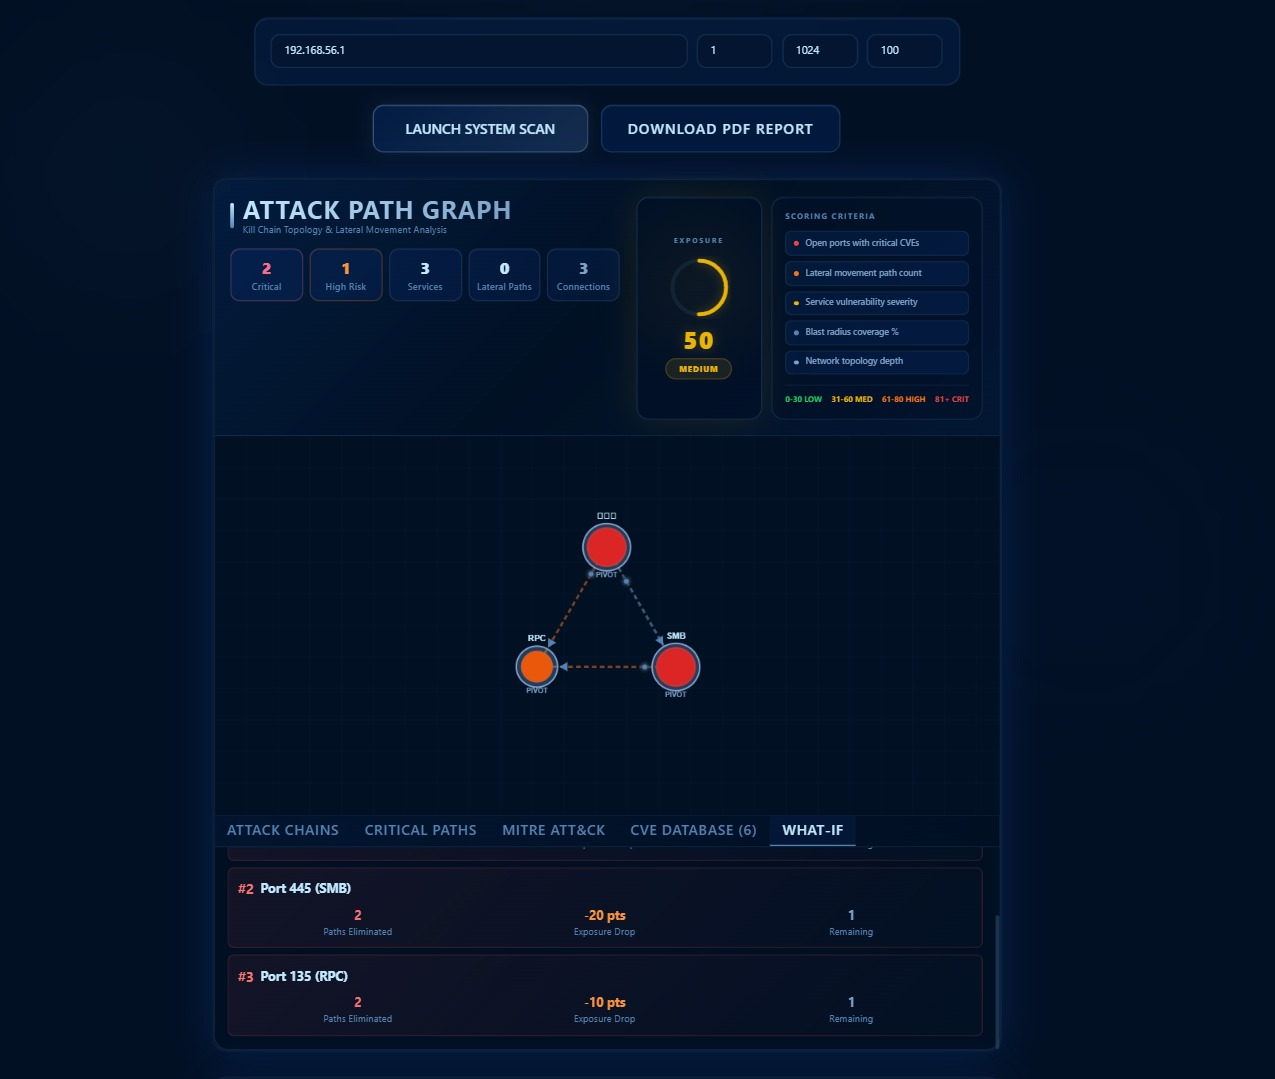
\includegraphics[width=\linewidth]{netC_whatif_netbios.jpg}
    \caption{What-If tab (view 1): \#1 Port 139 (NetBIOS) eliminates 2 paths ($-$20 pts, 1 remaining); \#2 Port 445 (SMB) eliminates 2 paths ($-$20 pts, 1 remaining). Attack graph shows BBB--RPC--SMB triangle topology with NES = 50 (Medium).}
    \label{fig:netC_whatif_netbios}
  \end{subfigure}
  \hfill
  \begin{subfigure}[b]{0.48\linewidth}
    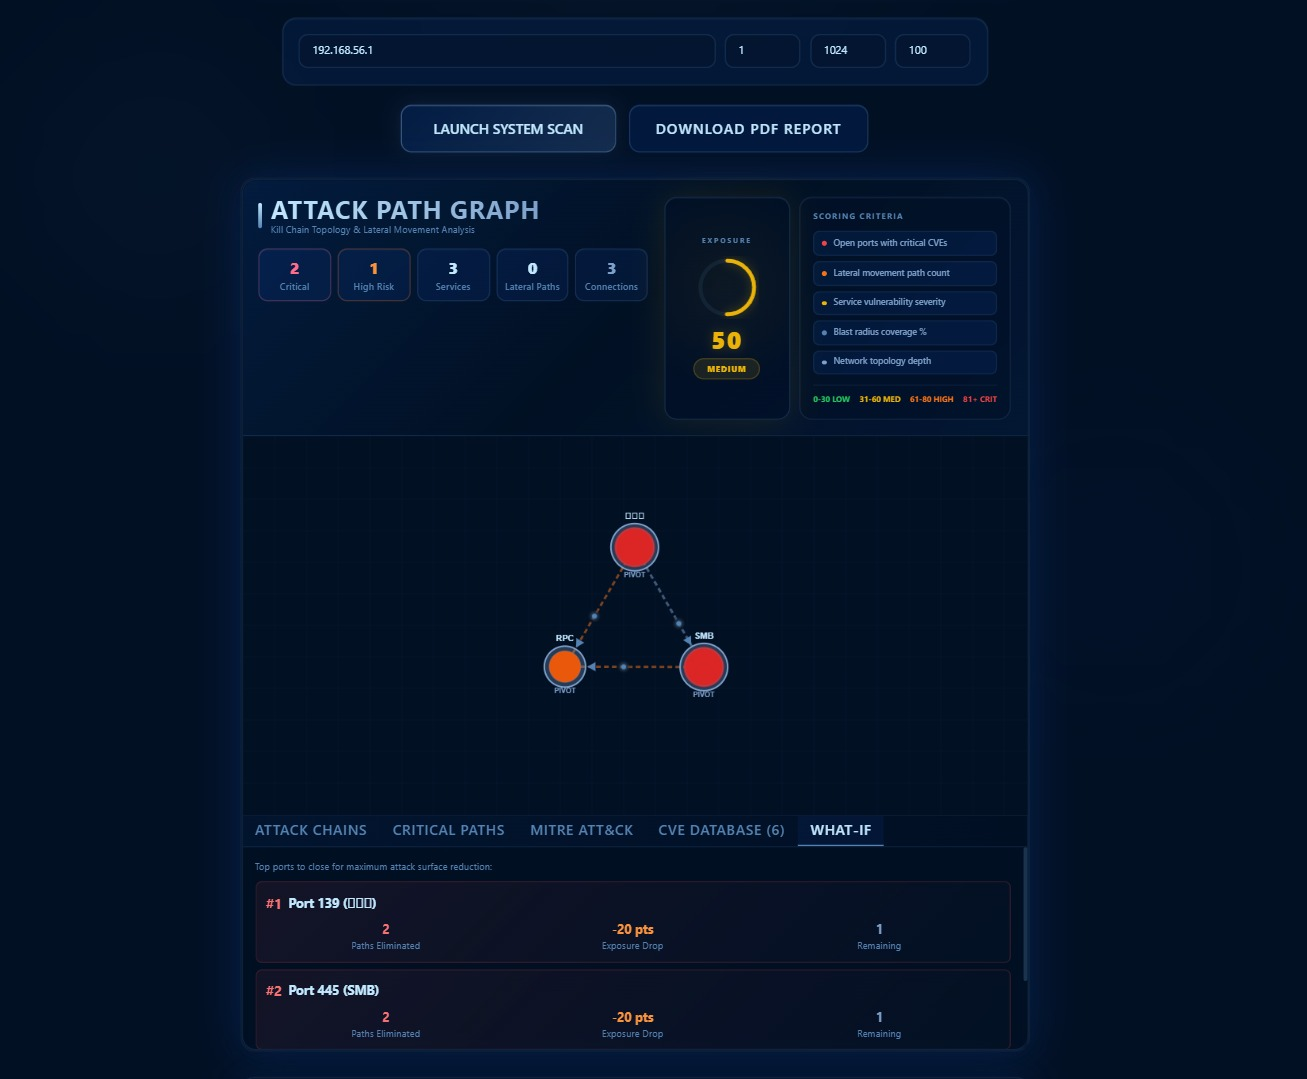
\includegraphics[width=\linewidth]{netC_whatif_smb.jpg}
    \caption{What-If tab (view 2): \#2 Port 445 (SMB) eliminates 2 paths ($-$20 pts, 1 remaining); \#3 Port 135 (RPC) eliminates 2 paths ($-$10 pts, 1 remaining). Confirms RPC as lowest-leverage remediation target.}
    \label{fig:netC_whatif_smb}
  \end{subfigure}
}
\caption{Network C (192.168.56.1) What-If mitigation analysis. The algorithm ranks ports according to their effectiveness at reducing the NES score: $-$20 pts for NetBIOS (Port 139) and SMB (Port 445), and $-$10 pts for RPC (Port 135).}
\label{fig:netC_whatif_full}
\end{figure}

% ============================================================
\subsubsection{Network D --- Mobile Hotspot Bridge (192.168.137.1)}
% ============================================================
Standard service connectivity was refused at the application layer. Zero open ports, CVEs, or attack paths were detected, confirming NES = 0.

% ============================================================
\subsubsection{Network E --- Public Internet Host 1 (208.67.222.222)}
% ============================================================
Network E represents the first internet-facing validation target and produced substantially richer results than the virtual lab environments. The platform identified \textbf{5 open ports} (21/FTP, 53/DNS, 80/HTTP, 179/BGP, 443/HTTPS), \textbf{6 CVEs}, \textbf{3 lateral paths}, and \textbf{3 inter-node connections}.

\begin{figure}[htbp]
\centerline{
  \begin{subfigure}[b]{0.48\linewidth}
    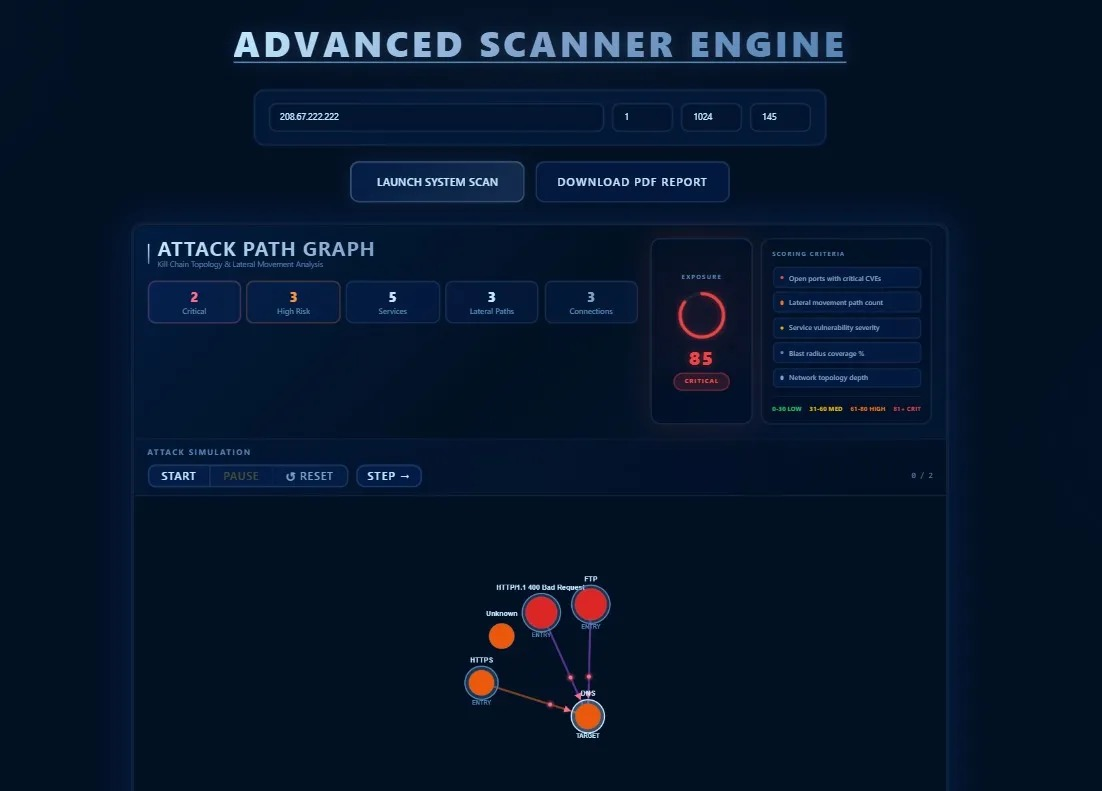
\includegraphics[width=\linewidth]{netE_dashboard.jpg}
    \caption{Network E dashboard: NES = 85 (Critical), 2 Critical nodes, 3 High Risk, 5 services, 3 lateral paths, 3 connections.}
    \label{fig:netE_dashboard}
  \end{subfigure}
  \hfill
  \begin{subfigure}[b]{0.48\linewidth}
    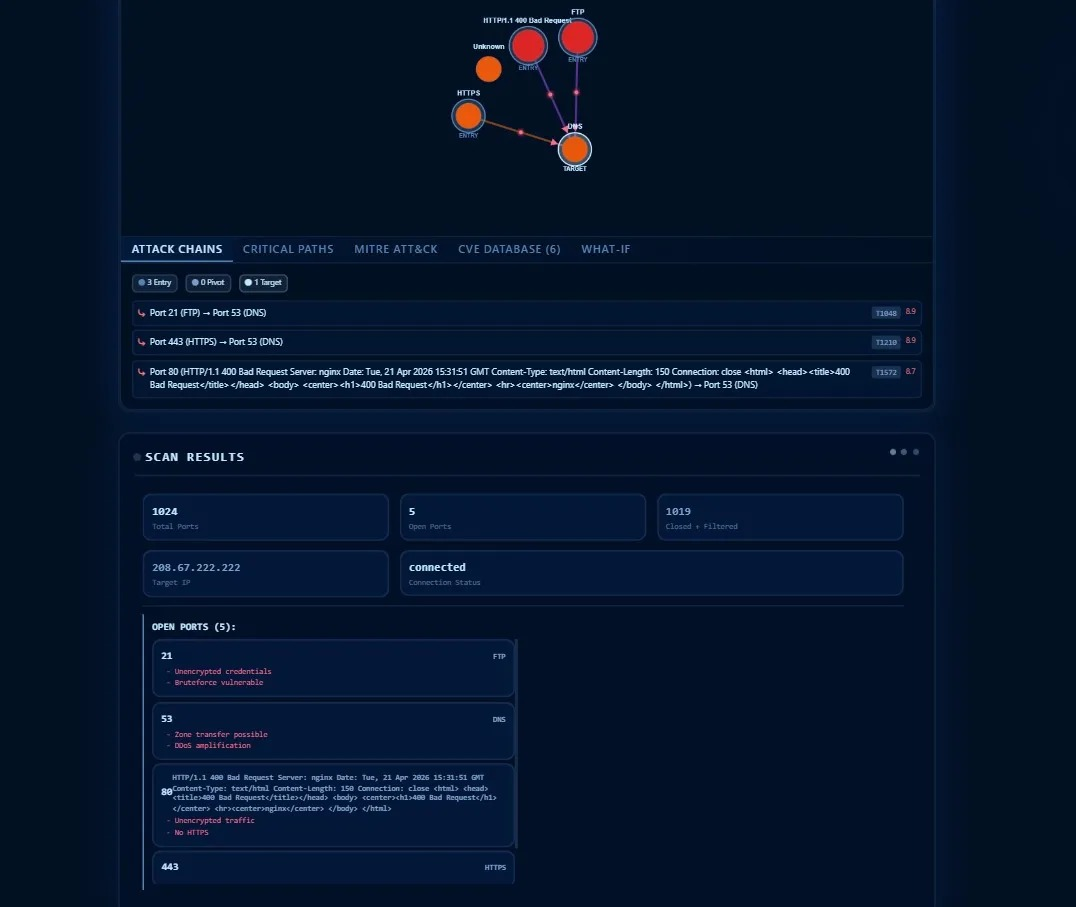
\includegraphics[width=\linewidth]{netE_scan.jpg}
    \caption{Scan results pane: 5 open ports including FTP (21), DNS (53), HTTP (80), HTTPS (443); attack chains visible.}
    \label{fig:netE_scan}
  \end{subfigure}
}
\caption{NET\_SCAN results for Network E (208.67.222.222). Five open ports, 3 lateral paths, NES = 85 (Critical).}
\label{fig:network_e_main}
\end{figure}

\begin{figure}[htbp]
\centerline{
  \begin{subfigure}[b]{0.48\linewidth}
    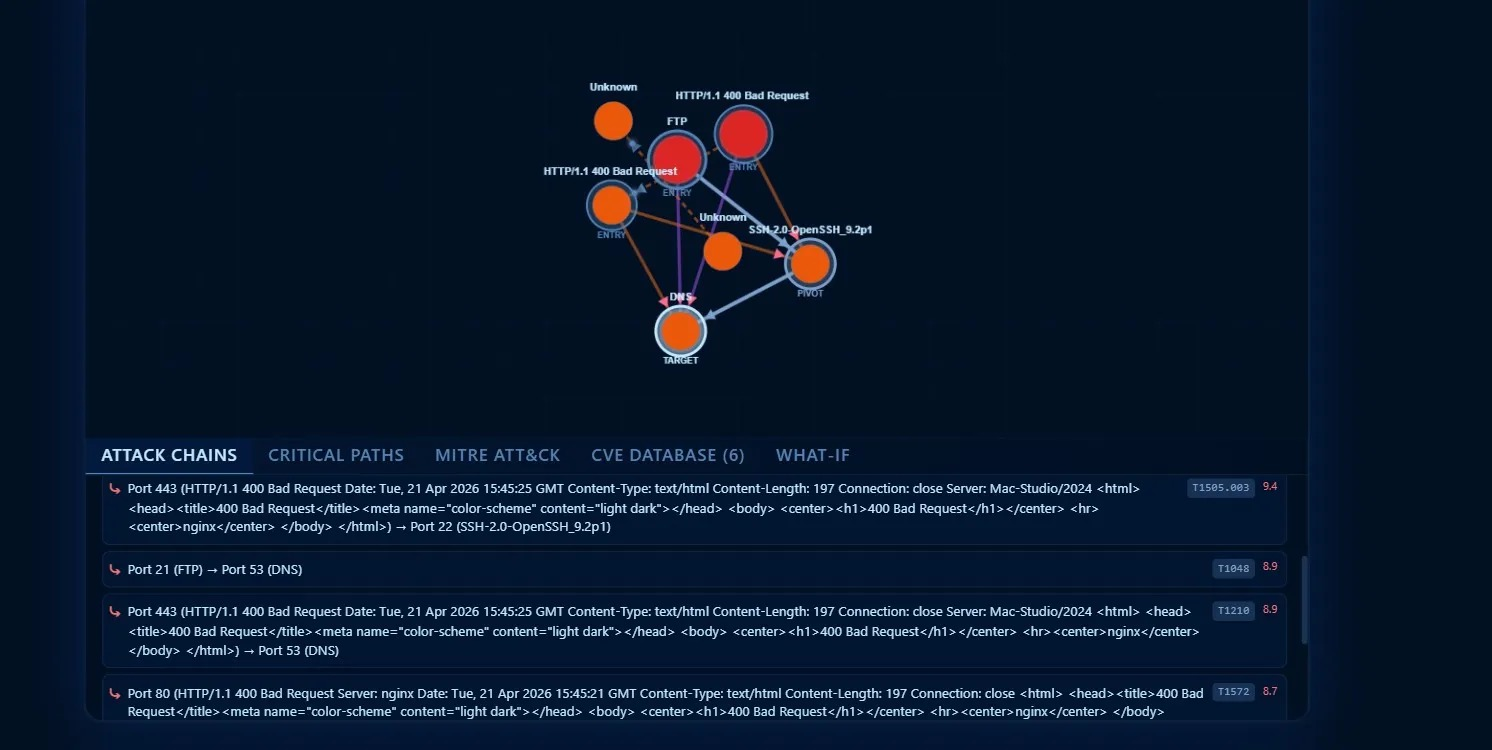
\includegraphics[width=\linewidth]{netE_chains1.jpg}
    \caption{Attack Chains tab (page 1): chains including Port 443 $\to$ Port 22 (SSH-2.0-OpenSSH\_9.2p1) with T1505.003 (Risk 9.4).}
    \label{fig:netE_chains1}
  \end{subfigure}
  \hfill
  \begin{subfigure}[b]{0.48\linewidth}
    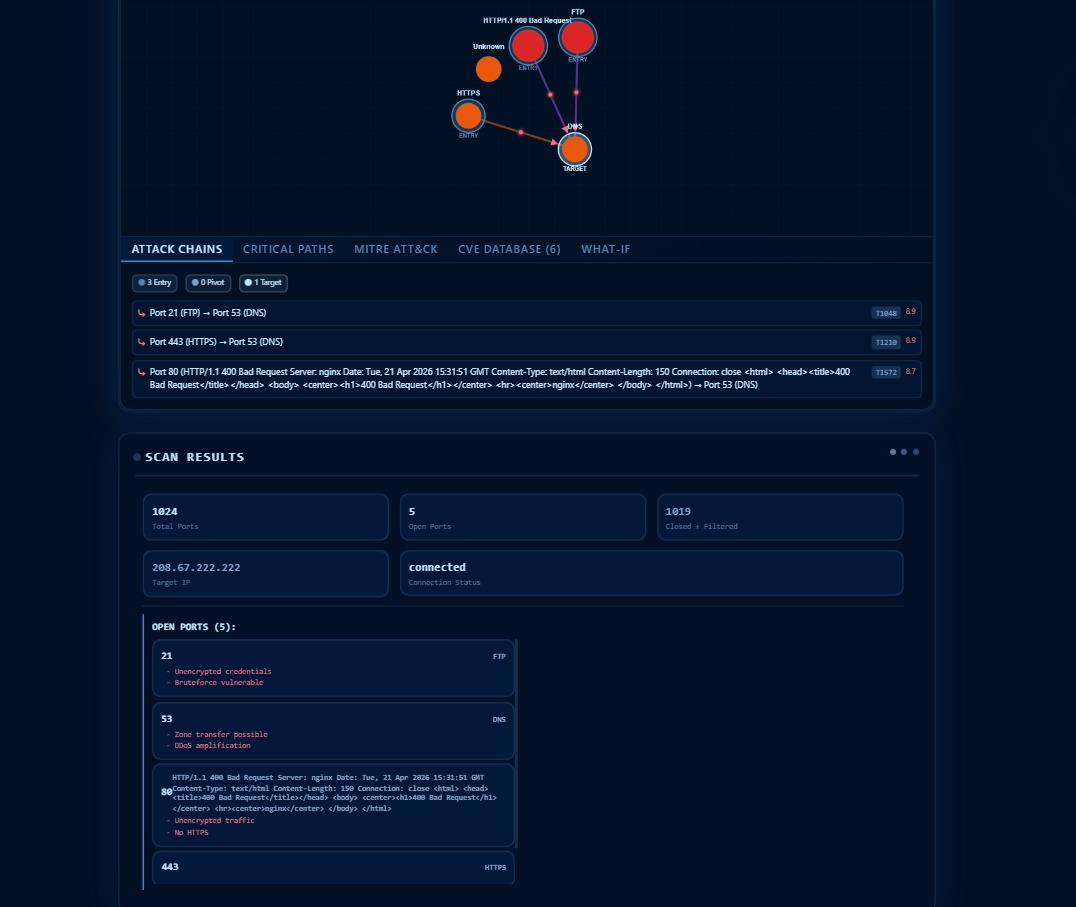
\includegraphics[width=\linewidth]{netE_chains2.jpg}
    \caption{Attack Chains tab (page 2): Port 80 $\to$ Port 53 (DNS) via T1572 (Risk 8.7) and Port 80 $\to$ Port 443 via T1210 (Risk 7.4).}
    \label{fig:netE_chains2}
  \end{subfigure}
}
\caption{Network E attack chain enumeration across all discovered services.}
\label{fig:netE_chains}
\end{figure}

\begin{figure}[htbp]
\centerline{
  \begin{subfigure}[b]{0.48\linewidth}
    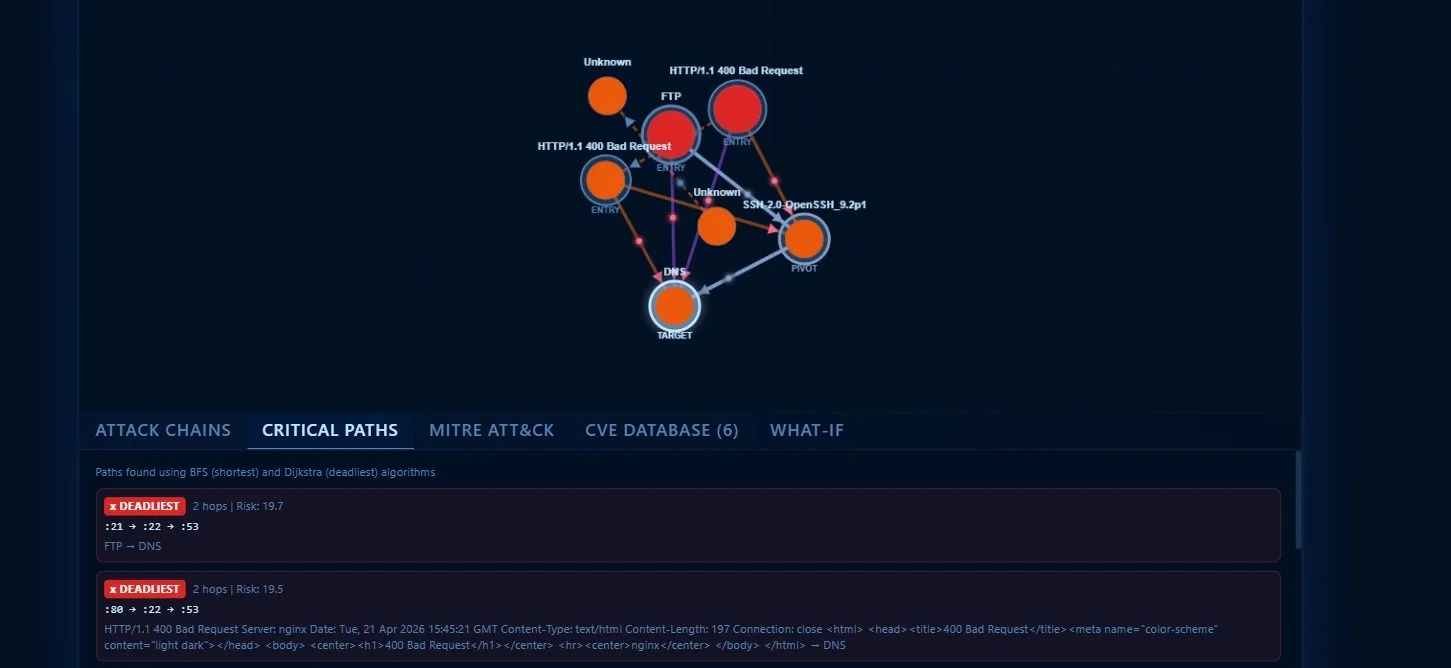
\includegraphics[width=\linewidth]{netE_critical1.jpg}
    \caption{Critical Paths (BFS/Dijkstra): \textsc{Deadliest} path :21$\to$:22$\to$:53 (FTP$\to$DNS, Risk 19.7); \textsc{Deadliest} :80$\to$:22$\to$:53 (Risk 19.5).}
    \label{fig:netE_crit1}
  \end{subfigure}
  \hfill
  \begin{subfigure}[b]{0.48\linewidth}
    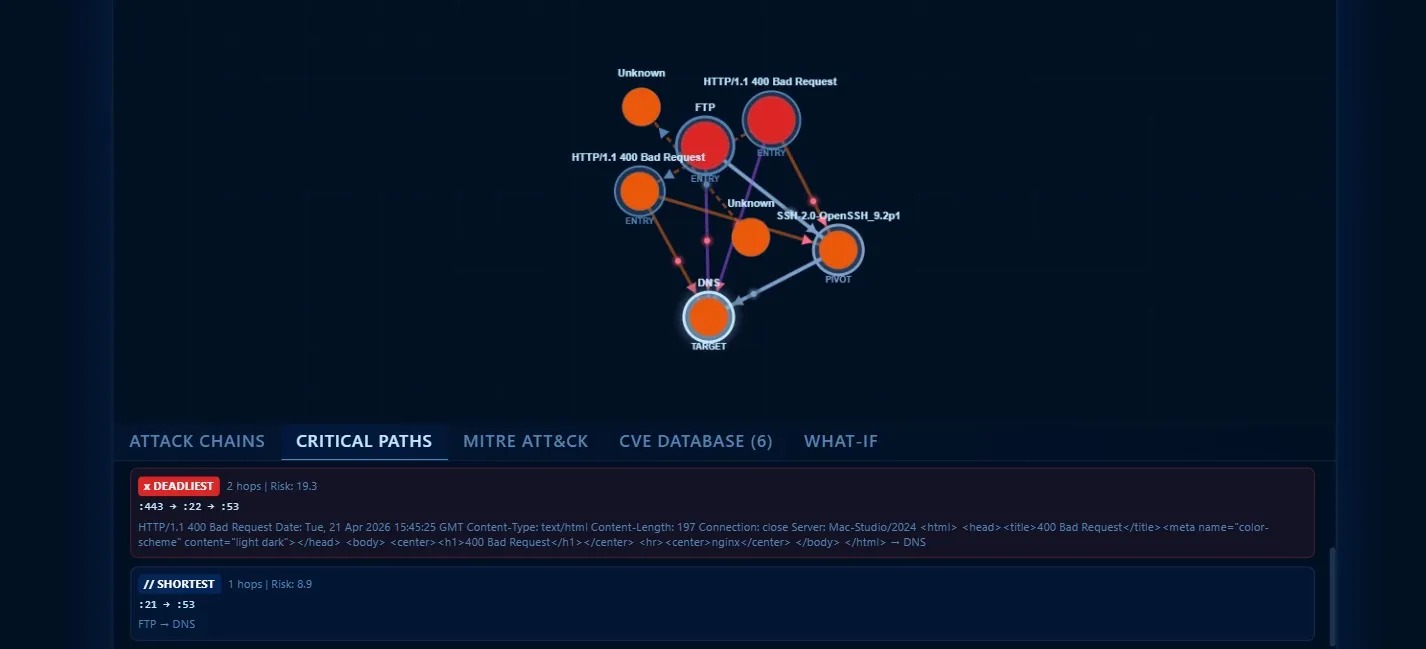
\includegraphics[width=\linewidth]{netE_critical2.jpg}
    \caption{Critical Paths (continued): \textsc{Deadliest} :443$\to$:22$\to$:53 (Risk 19.3); \textsc{Shortest} :443$\to$:53 (Risk 8.9, 1 hop).}
    \label{fig:netE_crit2}
  \end{subfigure}
}
\caption{Critical path analysis on Network E with BFS and Dijkstra algorithms, illustrating multi-hop kill chains via the SSH pivot node.}
\label{fig:netE_critical}
\end{figure}

\begin{figure}[htbp]
\centerline{
  \begin{subfigure}[b]{0.48\linewidth}
    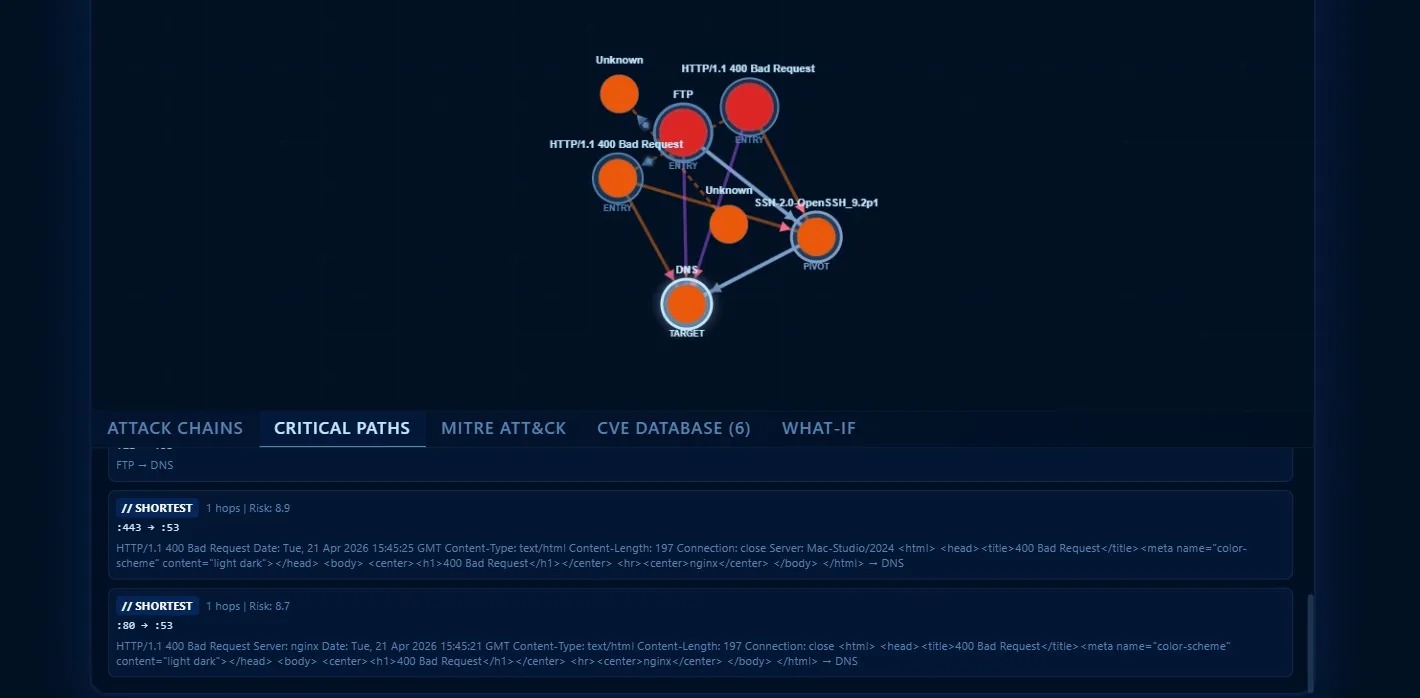
\includegraphics[width=\linewidth]{netE_critical3.jpg}
    \caption{Other critical paths such as :443$\to$:22$\to$:53 (most dangerous, Risk 19.3) and :21$\to$:53 (Shortest, Risk 8.9).}
    \label{fig:netE_crit3}
  \end{subfigure}
  \hfill
  \begin{subfigure}[b]{0.48\linewidth}
    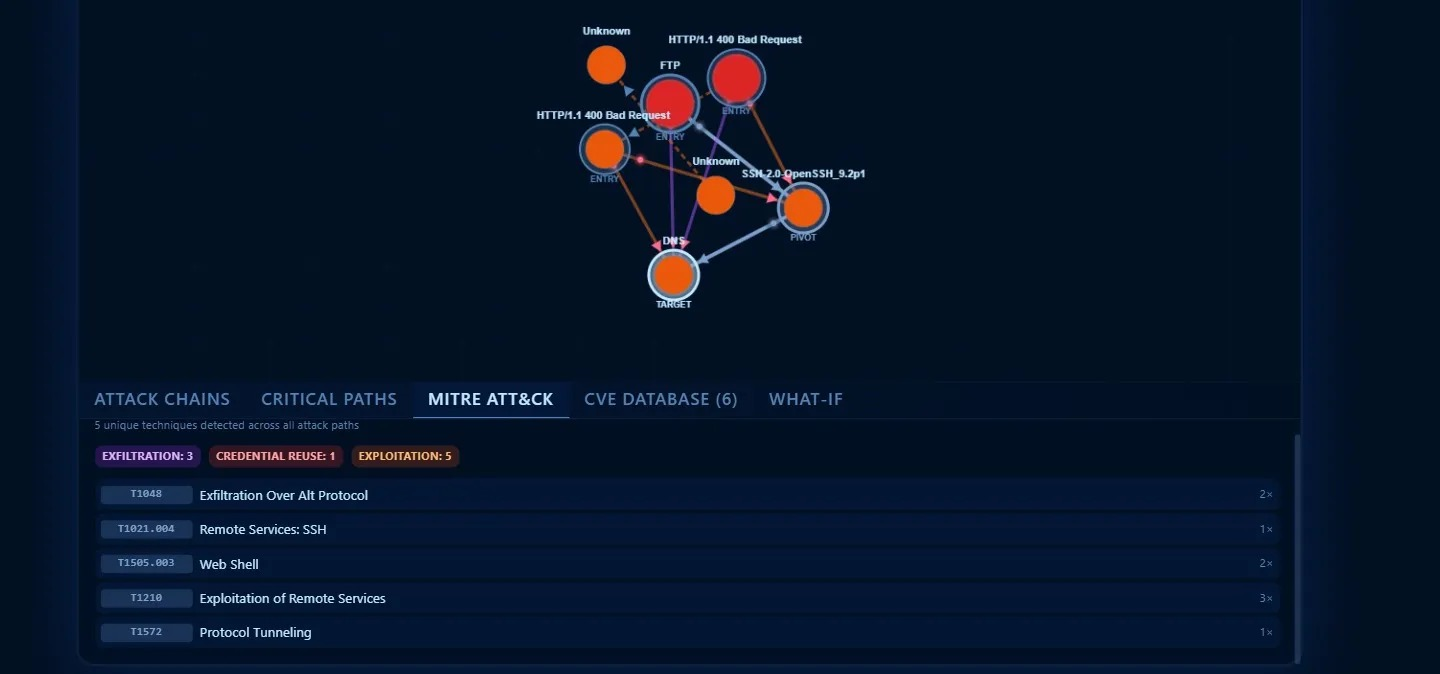
\includegraphics[width=\linewidth]{netE_mitre.jpg}
    \caption{MITRE ATT\&CK tab: 5 unique techniques detected---T1048, T1021.004, T1505.003, T1210, T1572.}
    \label{fig:netE_mitre}
  \end{subfigure}
}
\caption{Network E full critical path enumeration and MITRE ATT\&CK technique mapping.}
\label{fig:netE_full}
\end{figure}

The Critical Paths Engine identified three \textsc{Deadliest} paths (all 2-hop, Risk $\approx$ 19.3--19.7) routing through Port 22 (SSH-2.0-OpenSSH\_9.2p1) as a pivot node, and three \textsc{Shortest} paths (1-hop, Risk 8.7--8.9) directly reaching Port 53 (DNS) as the target. The MITRE ATT\&CK module identified \textbf{5 unique techniques}: T1048, T1021.004, T1505.003, T1210, and T1572.

\begin{table}[htbp]
\caption{Network E --- Critical Path Summary (BFS + Dijkstra)}
\begin{center}
\begin{tabular}{|l|l|c|c|}
\hline
\textbf{Type} & \textbf{Path} & \textbf{Hops} & \textbf{Risk} \\
\hline
\textsc{Deadliest} & :21 $\to$ :22 $\to$ :53 (FTP$\to$DNS) & 2 & 19.7 \\
\hline
\textsc{Deadliest} & :80 $\to$ :22 $\to$ :53 & 2 & 19.5 \\
\hline
\textsc{Deadliest} & :443 $\to$ :22 $\to$ :53 & 2 & 19.3 \\
\hline
\textsc{Shortest} & :443 $\to$ :53 (HTTPS$\to$DNS) & 1 & 8.9 \\
\hline
\textsc{Shortest} & :80 $\to$ :53 & 1 & 8.7 \\
\hline
\end{tabular}
\label{tab:paths_netE}
\end{center}
\end{table}

% ============================================================
\subsubsection{Network F --- Public Internet Host 2 (185.222.222.222)}
% ============================================================
Network F produced the highest-complexity scan across all environments, with NES reaching the platform ceiling of \textbf{100 (Critical)}. The results showed 7 services running, 9 connections between different systems, and 7 possible paths for lateral movement as well. Out of these, 2 of the nodes were flagged as critical and 5 as high risk.

\begin{figure}[htbp]
\centerline{
  \begin{subfigure}[b]{0.48\linewidth}
    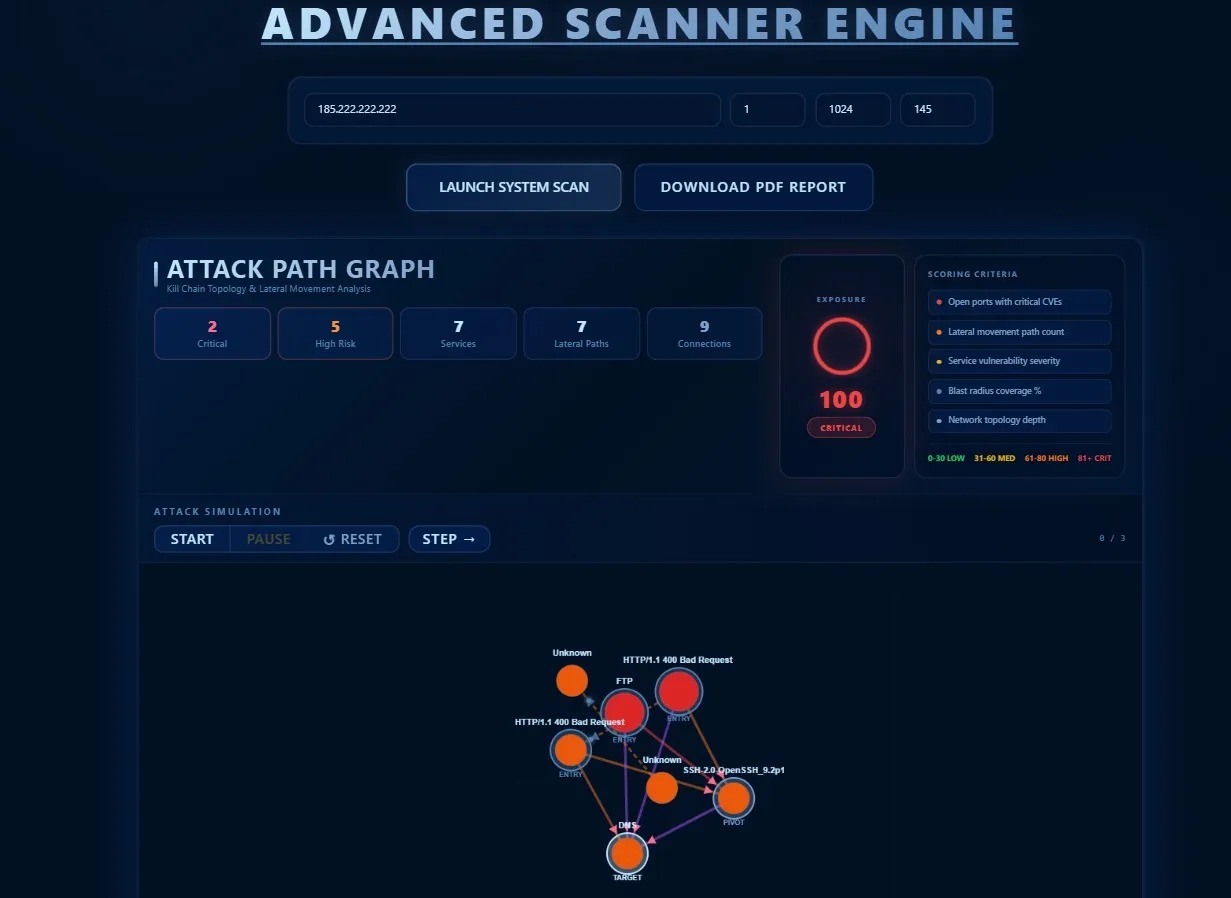
\includegraphics[width=\linewidth]{netF_dashboard.jpg}
    \caption{Network F dashboard: NES = 100 (Critical), 7 services, 7 lateral paths, 9 connections.}
    \label{fig:netF_dashboard}
  \end{subfigure}
  \hfill
  \begin{subfigure}[b]{0.48\linewidth}
    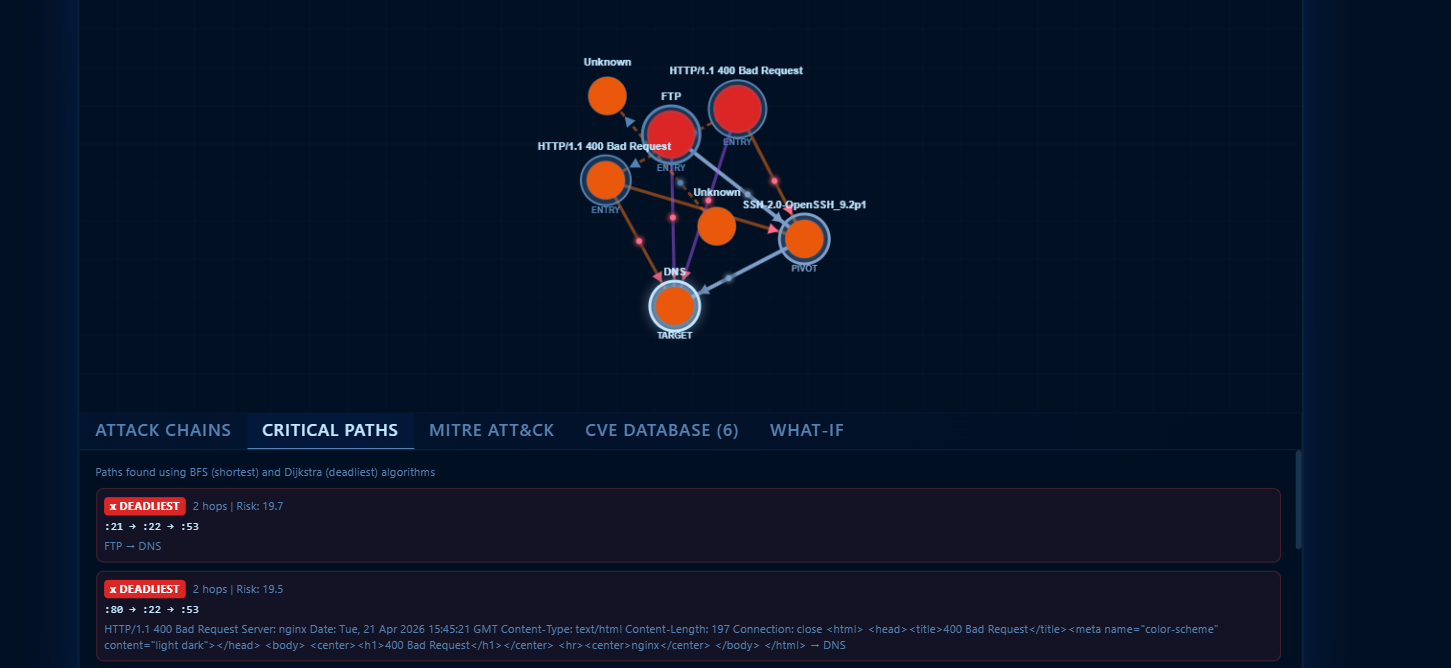
\includegraphics[width=\linewidth]{netF_critical1.jpg}
    \caption{Critical paths: shortest chains including :21$\to$:53, :443$\to$:53, :80$\to$:53 (Risk 8.7--8.9, 1 hop).}
    \label{fig:netF_crit1}
  \end{subfigure}
}
\caption{Network F (185.222.222.222) main dashboard and critical path enumeration. NES saturates at 100 (Critical).}
\label{fig:network_f_main}
\end{figure}

\begin{figure}[htbp]
\centerline{
  \begin{subfigure}[b]{0.48\linewidth}
    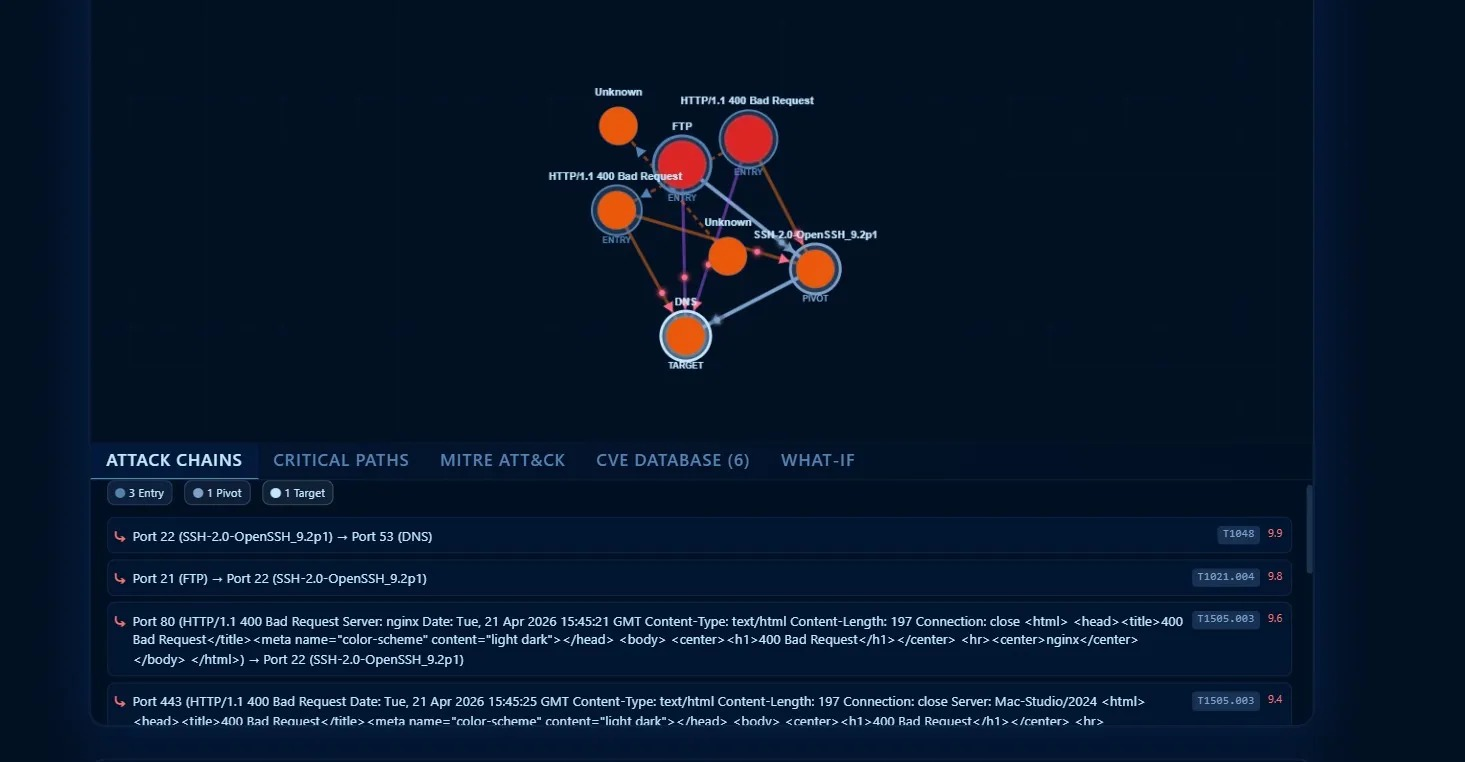
\includegraphics[width=\linewidth]{netF_chains.jpg}
    \caption{Network F Attack Chains tab: 3 Entry nodes, 1 Pivot, 1 Target; chains including Port 22 (SSH-2.0-OpenSSH\_9.2p1) $\to$ Port 53 (DNS) via T1048 (Risk 9.9) and Port 21 (FTP) $\to$ Port 22 via T1021.004 (Risk 9.8).}
    \label{fig:netF_chains}
  \end{subfigure}
  \hfill
  \begin{subfigure}[b]{0.48\linewidth}
    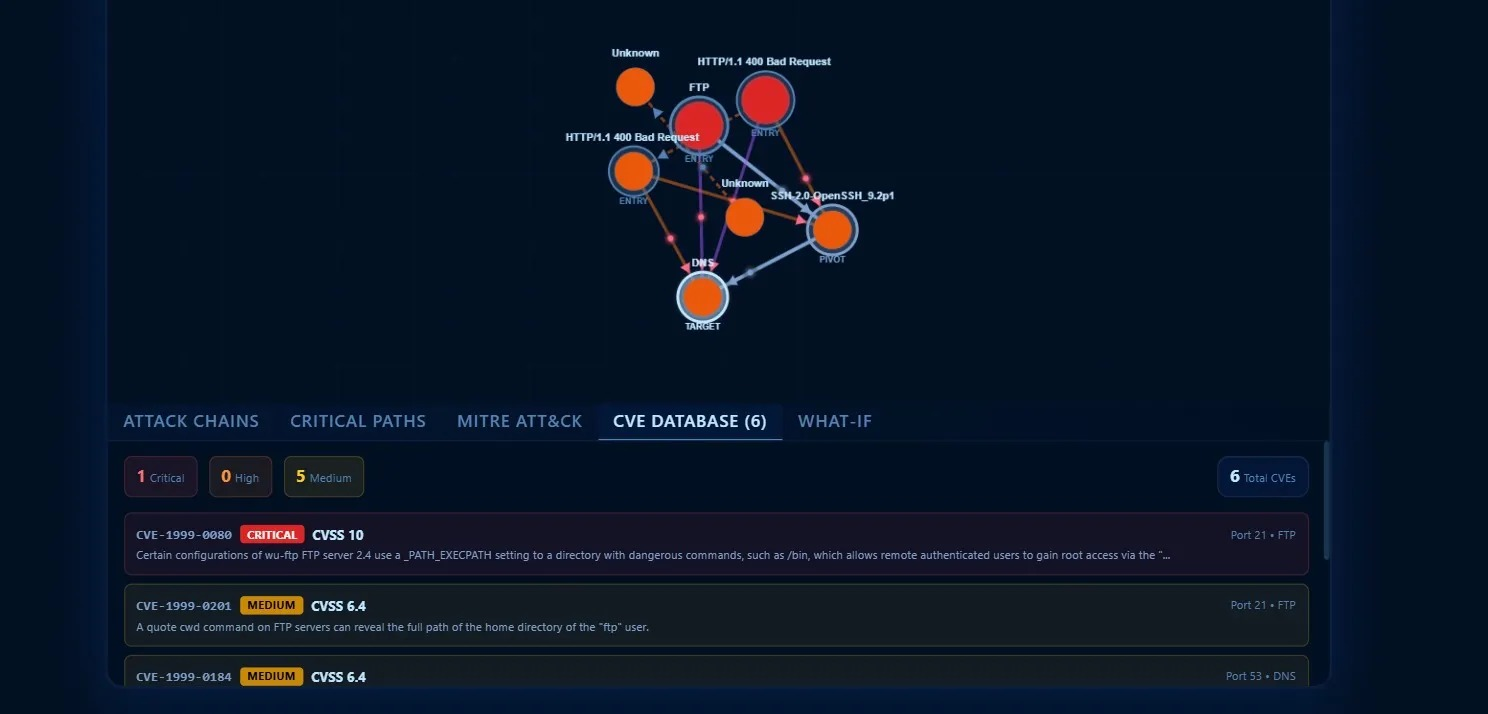
\includegraphics[width=\linewidth]{netF_cve.jpg}
    \caption{CVE Database tab (6 total): 1 Critical (CVE-1999-0080, CVSS 10.0, FTP), 0 High, 5 Medium; CVE-1999-0201 (CVSS 6.4, FTP) and CVE-1999-0184 (CVSS 6.4, DNS) visible.}
    \label{fig:netF_cve}
  \end{subfigure}
}
\caption{Network F attack chain enumeration and CVE database breakdown.}
\label{fig:netF_chains_cve}
\end{figure}

\begin{figure}[htbp]
\centerline{
  \begin{subfigure}[b]{0.48\linewidth}
    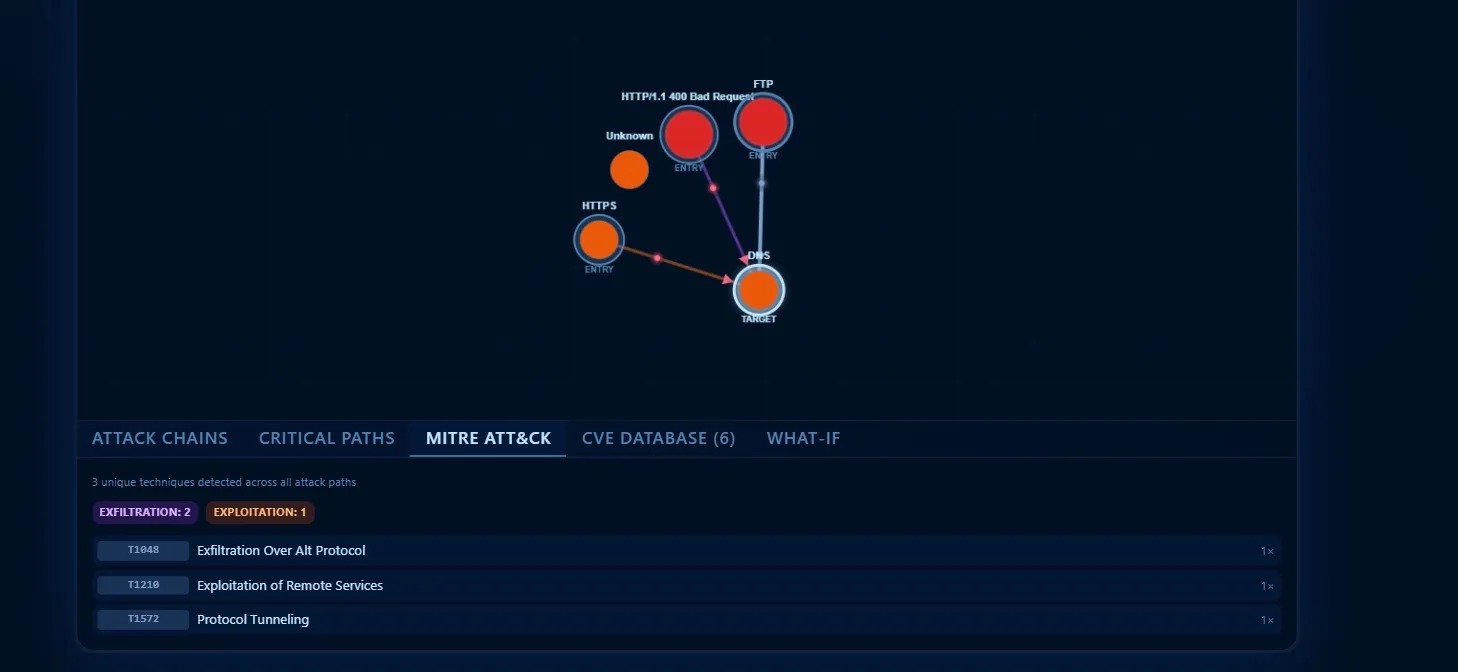
\includegraphics[width=\linewidth]{netF_mitre.jpg}
    \caption{MITRE ATT\&CK: 3 unique techniques---T1048 (Exfiltration Over Alt Protocol, $1\times$), T1210 ($1\times$), T1572 ($1\times$).}
    \label{fig:netF_mitre}
  \end{subfigure}
  \hfill
  \begin{subfigure}[b]{0.48\linewidth}
    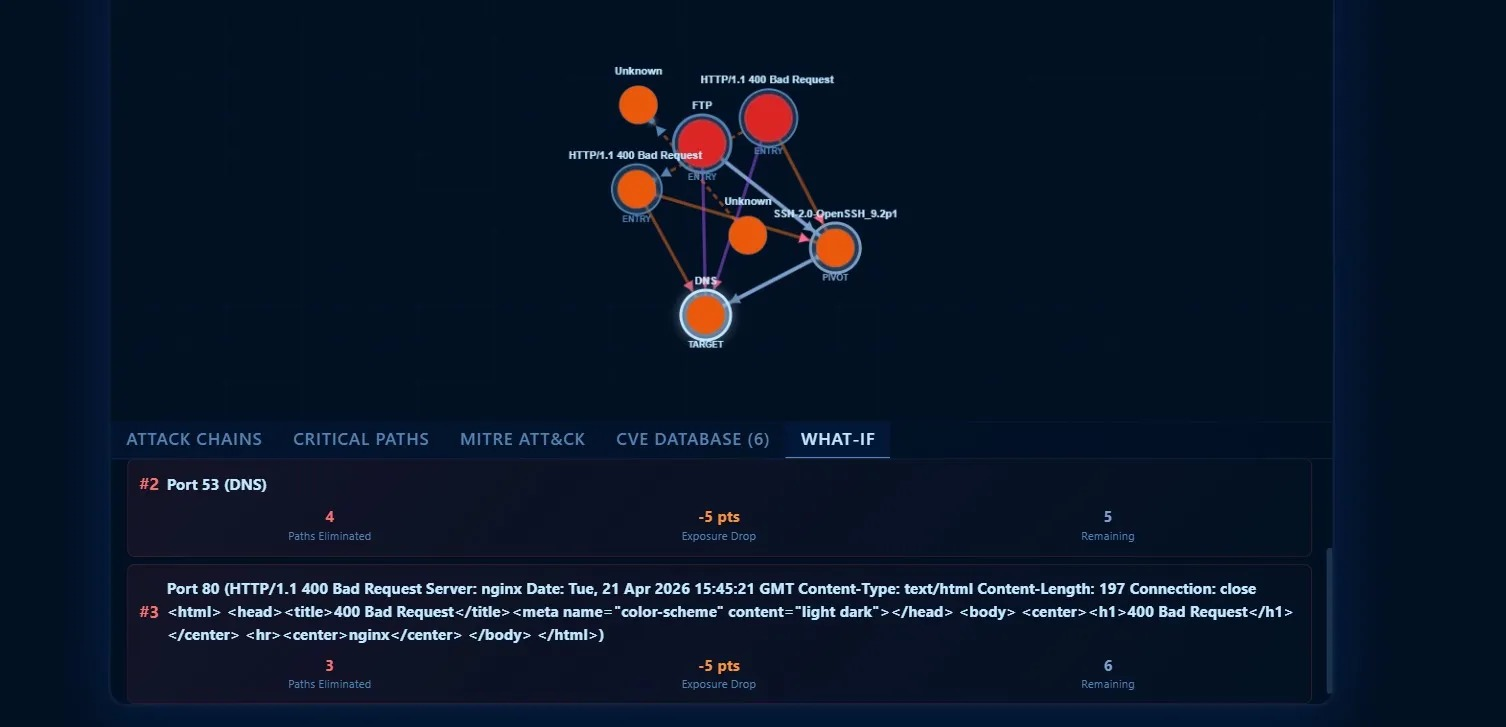
\includegraphics[width=\linewidth]{netF_whatif.jpg}
    \caption{What-If tab: removing Port 53 (DNS) eliminates 4 paths ($-$5 pts, 5 remaining); removing Port 80 (nginx 400 Bad Request) eliminates 3 paths ($-$5 pts, 6 remaining).}
    \label{fig:netF_whatif}
  \end{subfigure}
}
\caption{Network F MITRE ATT\&CK mapping and What-If mitigation analysis.}
\label{fig:netF_analysis}
\end{figure}

The CVE database for Network F comprised \textbf{6 CVEs} (1 Critical, 0 High, 5 Medium). The most severe was CVE-1999-0080 (CVSS 10.0, Critical), associated with Port 21 (FTP), which allows remote authenticated users to gain root access via wu-ftp PATH\_EXECPATH misconfiguration. The What-If analysis revealed that removing Port 53 (DNS) eliminates 4 lateral paths and reduces NES by 5 points (7 remaining). Removing Port 80 (nginx) eliminates 3 further paths ($-$5 pts). These results confirm DNS as the highest-leverage remediation target in this topology.

\begin{table}[htbp]
\caption{Network F --- Detailed Scan Summary (185.222.222.222)}
\begin{center}
\begin{tabular}{|l|c|}
\hline
\textbf{Parameter} & \textbf{Value} \\
\hline
Target IP & 185.222.222.222 \\
\hline
Open Ports & 7+ (21, 53, 80, 179, 443, 853+) \\
\hline
CVEs Identified & 6 (1 Critical, 0 High, 5 Medium) \\
\hline
Critical Nodes & 2 \\
\hline
High Risk Nodes & 5 \\
\hline
Attack Path Connections & 9 \\
\hline
Lateral Paths & 7 \\
\hline
MITRE Techniques Mapped & 3 (T1048, T1210, T1572) \\
\hline
\textbf{NES Score} & \textbf{100 -- Critical} \\
\hline
\end{tabular}
\label{tab:netF_detail}
\end{center}
\end{table}

% ============================================================
\subsubsection{Network G --- Local SMB Host (172.20.10.3)}
% ============================================================
Network G targeted the scanning host's own Wi-Fi adapter (172.20.10.3), which exposes Windows file-sharing services on the local subnet. The system found \textbf{3 open ports}: Port 135 (RPC), Port 139 (NetBIOS/SMB exploitation vector), and Port 445 (SMB, ransomware propagation vector). Six CVEs were correlated. The heuristic engine classified 2 Critical nodes and 1 High Risk node, with 3 inter-service connections and \textbf{0 lateral paths}---reflecting that while individual services carry high CVE severity, the absence of pivotable paths limits compounded topological risk.

The NES engine computed a score of \textbf{50 (Medium)}, consistent with Network C (also 3 services, 0 lateral paths). The attack graph rendered a triangle topology: RPC $\leftrightarrow$ NetBIOS $\leftrightarrow$ SMB, all classified as Entry nodes with RPC as the pivot gateway. Two MITRE techniques were mapped: T1136 (Create Account, associated with NetBIOS exploitation) and T1210 (Exploitation of Remote Services, associated with SMB lateral movement).

\begin{figure}[htbp]
\centerline{
  \begin{subfigure}[b]{0.48\linewidth}
    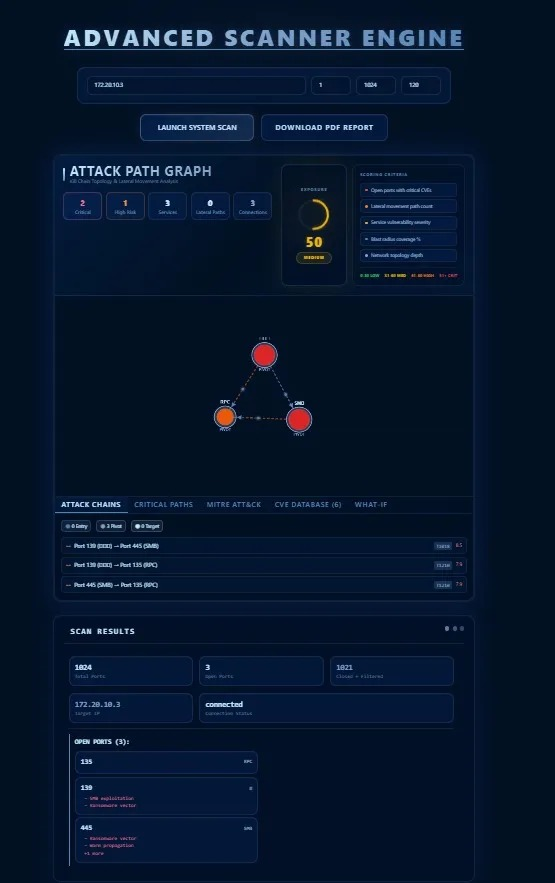
\includegraphics[width=\linewidth]{netG_dashboard.jpg}
    \caption{Network G dashboard (172.20.10.3): NES = 50 (Medium), 2 Critical + 1 High Risk nodes, 3 services, 0 lateral paths, 3 connections. Open ports: 135 (RPC), 139 (NetBIOS/B), 445 (SMB).}
    \label{fig:netG_dashboard}
  \end{subfigure}
  \hfill
  \begin{subfigure}[b]{0.48\linewidth}
    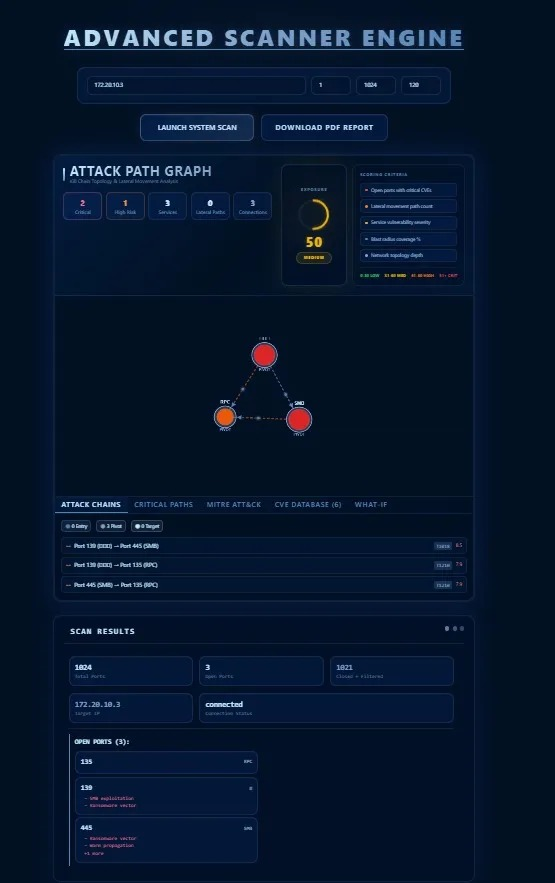
\includegraphics[width=\linewidth]{netG_dashboard2.jpg}
    \caption{Network G attack graph and scan results: 1024 ports scanned, 3 open, 1021 closed/filtered. Attack chains showing Port 139 (B) $\to$ Port 445 (SMB) via T1136, and Port 445 (SMB) $\to$ Port 135 (RPC) via T1210.}
    \label{fig:netG_scan}
  \end{subfigure}
}
\caption{NET\_SCAN results for Network G (172.20.10.3). Three open Windows file-sharing ports, NES = 50 (Medium).}
\label{fig:network_g_main}
\end{figure}

\begin{table}[htbp]
\caption{Network G --- Detailed Scan Summary (172.20.10.3)}
\begin{center}
\begin{tabular}{|l|c|}
\hline
\textbf{Parameter} & \textbf{Value} \\
\hline
Target IP & 172.20.10.3 \\
\hline
Connection Status & Connected \\
\hline
Total Ports Scanned & 1024 \\
\hline
Open Ports & 3 (135/RPC, 139/B, 445/SMB) \\
\hline
Closed / Filtered & 1021 \\
\hline
CVEs Identified & 6 \\
\hline
Critical Nodes & 2 \\
\hline
High Risk Nodes & 1 \\
\hline
Attack Path Connections & 3 \\
\hline
Lateral Paths & 0 \\
\hline
MITRE Techniques Mapped & 2 (T1136, T1210) \\
\hline
\textbf{NES Score} & \textbf{50 -- Medium} \\
\hline
\end{tabular}
\label{tab:netG_detail}
\end{center}
\end{table}

% ============================================================
\subsubsection{Network H --- Google Public DNS (8.8.8.8)}
% ============================================================
Network H targeted \texttt{8.8.8.8}, a globally distributed anycast public DNS resolver operated by Google, to assess NET\_SCAN's behavior against a well-known, operationally hardened internet host. This scan produced the \textbf{High} risk tier---NES = \textbf{60}---making it the only environment in the test suite to occupy the High band (60--80), positioned between the Medium environments (Networks C and G, NES = 50) and the Critical environments (Networks E and F).

The system identify \textbf{4 open services}: Port 21 (FTP), Port 53 (DNS), Port 443 (HTTPS, returning HTTP/400 Bad Request) and Port 853 (DNS-over-TLS). Six CVEs were enriched from NVD. The attack graph rendered 1 Critical node, 3 High Risk nodes, \textbf{2 lateral paths}, and \textbf{3 inter-node connections}.

\begin{figure}[htbp]
\centerline{
  \begin{subfigure}[b]{0.48\linewidth}
    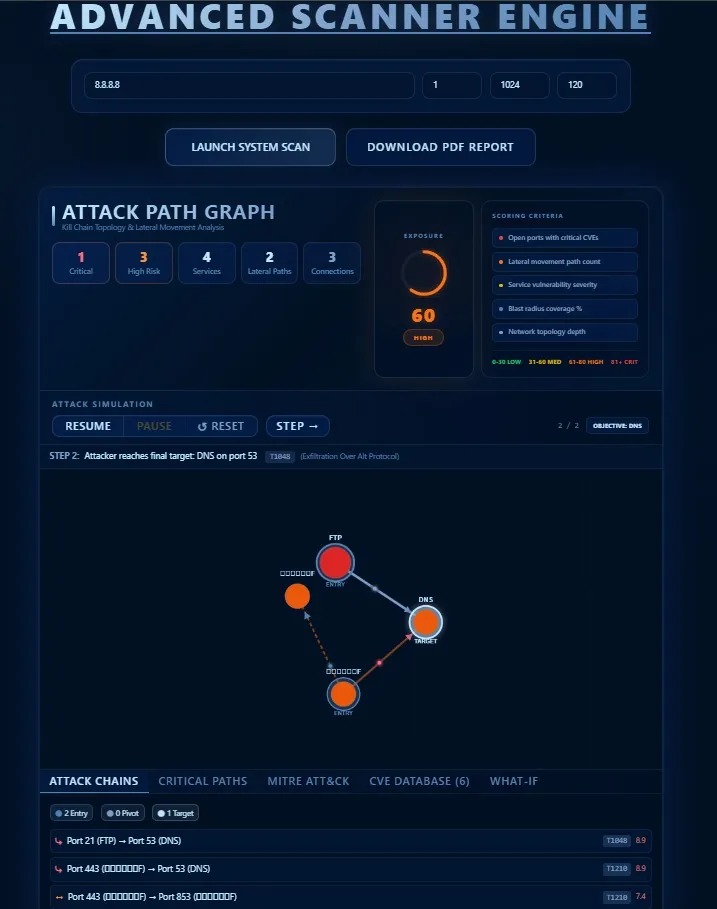
\includegraphics[width=\linewidth]{netH_dashboard.jpg}
    \caption{Network H dashboard (8.8.8.8): NES = 60 (High), 1 Critical + 3 High Risk nodes, 4 services, 2 lateral paths, 3 connections.}
    \label{fig:netH_dashboard}
  \end{subfigure}
  \hfill
  \begin{subfigure}[b]{0.48\linewidth}
    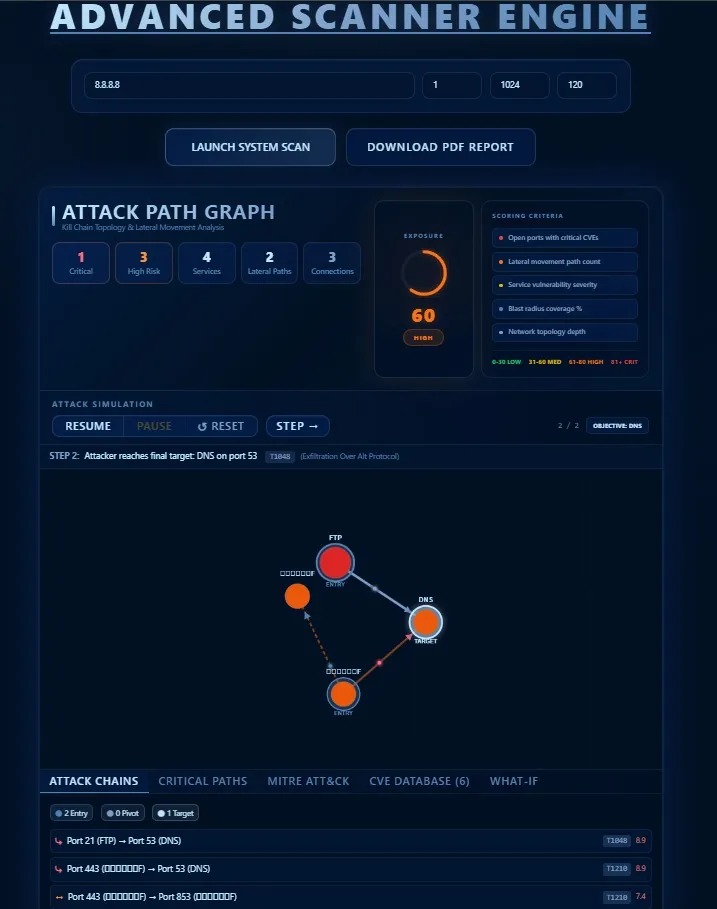
\includegraphics[width=\linewidth]{netH_chains.jpg}
    \caption{Attack Chains tab: 2 Entry nodes, 0 Pivot, 1 Target. Chains: Port 21 (FTP) $\to$ Port 53 (DNS) via T1048 (Risk 8.9); Port 443 $\to$ Port 53 via T1210 (Risk 8.9); Port 443 $\to$ Port 853 via T1210 (Risk 7.4).}
    \label{fig:netH_chains}
  \end{subfigure}
}
\caption{NET\_SCAN results for Network H (8.8.8.8). Four services, 2 lateral paths, NES = 60 (High).}
\label{fig:network_h_main}
\end{figure}

\begin{figure}[htbp]
\centerline{
  \begin{subfigure}[b]{0.48\linewidth}
    
\includegraphics[width=\linewidth]{netH_critical.jpg}
    \caption{Critical Paths (BFS): two \textsc{Shortest} paths: :21$\to$:53 (FTP$\to$DNS, 1 hop, Risk 8.9) and :443$\to$:53 (HTTPS$\to$DNS, 1 hop, Risk 8.9). Attack simulation at Step 1: initial access through FTP on port 21.}
    \label{fig:netH_crit1}
  \end{subfigure}
  \hfill
  \begin{subfigure}[b]{0.48\linewidth}
    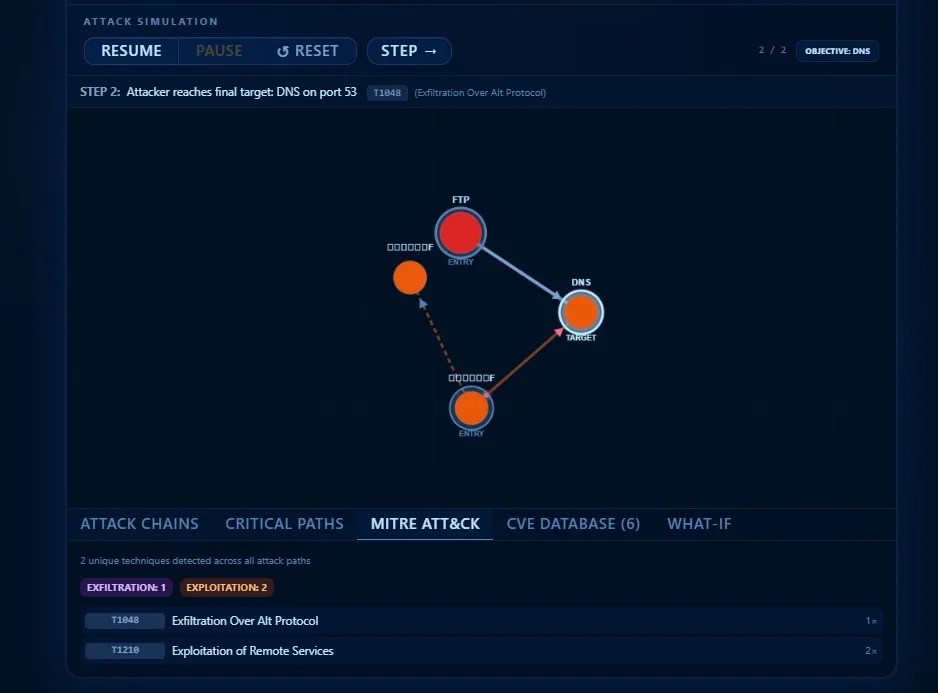
\includegraphics[width=\linewidth]{netH_critical2.jpg}
    \caption{Attack simulation Step 2: attacker reaches final target DNS on port 53 via T1048 (Exfiltration Over Alt Protocol). Both paths confirm DNS as the sole Target node.}
    \label{fig:netH_crit2}
  \end{subfigure}
}
\caption{Network H critical path analysis (BFS): direct 1-hop routes to DNS Target from FTP and HTTPS Entry nodes.}
\label{fig:netH_critical}
\end{figure}

\begin{figure}[htbp]
\centerline{
  \begin{subfigure}[b]{0.48\linewidth}
    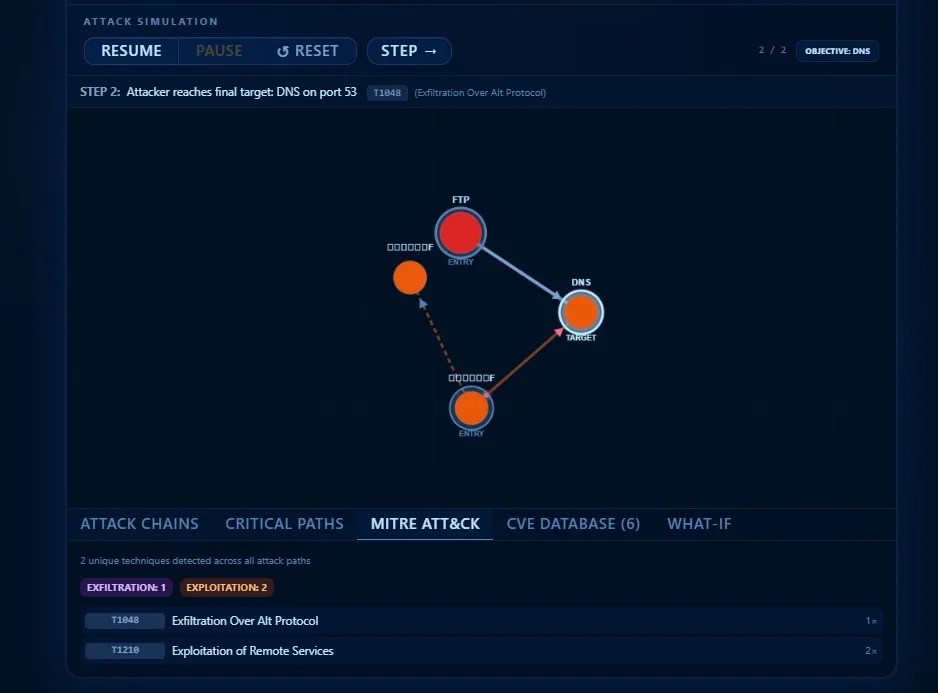
\includegraphics[width=\linewidth]{netH_critical3.jpg}
    \caption{Network H full dashboard view: NES = 60 (High), attack simulation complete (2/2 steps), scoring criteria visible including open ports with critical CVEs, lateral movement path count, and blast radius coverage.}
    \label{fig:netH_crit3}
  \end{subfigure}
  \hfill
  \begin{subfigure}[b]{0.48\linewidth}
    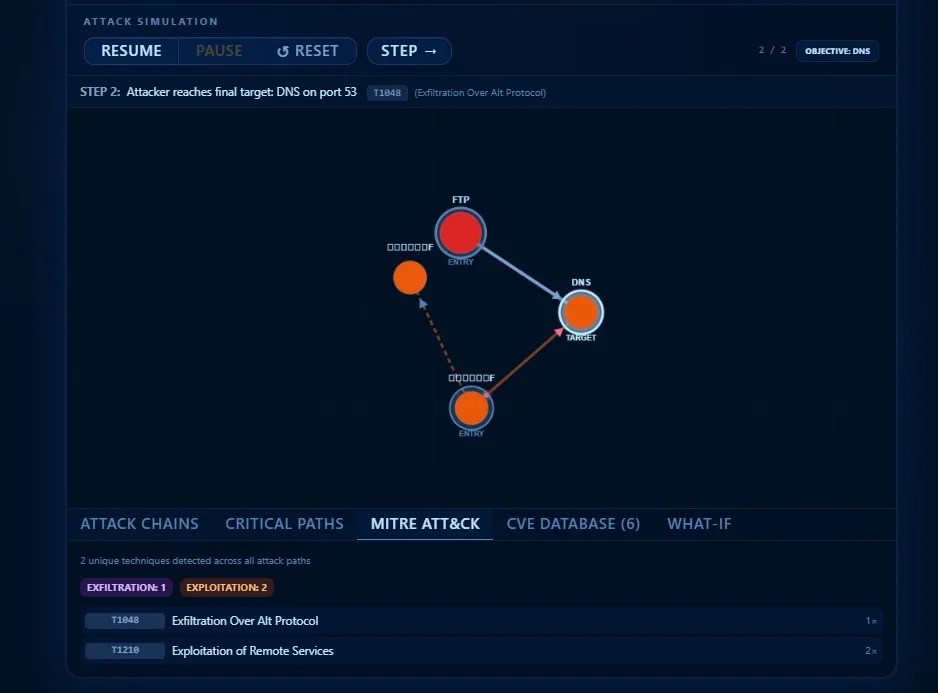
\includegraphics[width=\linewidth]{netH_mitre.jpg}
    \caption{MITRE ATT\&CK tab: 2 unique techniques across all attack paths---T1048 (Exfiltration Over Alt Protocol, Exfiltration category, $1\times$) and T1210 (Exploitation of Remote Services, Exploitation category, $2\times$).}
    \label{fig:netH_mitre}
  \end{subfigure}
}
\caption{Network H full-platform view and MITRE ATT\&CK technique mapping.}
\label{fig:netH_full}
\end{figure}

The Critical Paths Engine found exclusively \textsc{Shortest} paths with no \textsc{Deadliest} divergence, indicating that for 8.8.8.8's topology the shortest-hop and highest-risk traversals are identical. Both paths (Risk 8.9) route directly from FTP or HTTPS Entry nodes to DNS as the Target in a single hop. The MITRE ATT\&CK module identified \textbf{2 unique techniques}: T1048 (Exfiltration Over Alt Protocol, $1\times$) and T1210 (Exploitation of Remote Services, $2\times$), spanning Exfiltration (1) and Exploitation (2) categories.

A notable observation is that despite 8.8.8.8's operational reputation as a hardened global resolver, NET\_SCAN classified its exposure as High (NES = 60)---above the Medium tier of the local SMB host (Network G, NES = 50)---due to the presence of 2 lateral paths versus Network G's 0 lateral paths. This result illustrates that topological path availability is a more decisive NES driver than raw CVE count alone at the Medium--High boundary.

\begin{table}[htbp]
\caption{Network H --- Critical Path Summary (BFS)}
\begin{center}
\begin{tabular}{|l|l|c|c|}
\hline
\textbf{Type} & \textbf{Path} & \textbf{Hops} & \textbf{Risk} \\
\hline
\textsc{Shortest} & :21 $\to$ :53 (FTP $\to$ DNS) & 1 & 8.9 \\
\hline
\textsc{Shortest} & :443 $\to$ :53 (HTTPS $\to$ DNS) & 1 & 8.9 \\
\hline
\end{tabular}
\label{tab:paths_netH}
\end{center}
\end{table}

\begin{table}[htbp]
\caption{Network H --- Detailed Scan Summary (8.8.8.8)}
\begin{center}
\begin{tabular}{|l|c|}
\hline
\textbf{Parameter} & \textbf{Value} \\
\hline
Target IP & 8.8.8.8 \\
\hline
Connection Status & Connected \\
\hline
Total Ports Scanned & 1024 \\
\hline
Open Ports & 4 (21/FTP, 53/DNS, 443/HTTPS, 853/DoT) \\
\hline
CVEs Identified & 6 \\
\hline
Critical Nodes & 1 \\
\hline
High Risk Nodes & 3 \\
\hline
Attack Path Connections & 3 \\
\hline
Lateral Paths & 2 \\
\hline
MITRE Techniques Mapped & 2 (T1048, T1210) \\
\hline
\textbf{NES Score} & \textbf{60 -- High} \\
\hline
\end{tabular}
\label{tab:netH_detail}
\end{center}
\end{table}

\subsection{Comparative Exposure Analysis}
The eight-network validation demonstrates NET\_SCAN's adaptive scoring across a full spectrum of exposure profiles from clean isolated interfaces to maximally exposed internet-facing hosts.

\begin{table}[htbp]
\caption{Comparative NES Scoring Breakdown Across All Eight Networks}
\begin{center}
\begin{tabular}{|l|c|c|c|c|c|c|c|c|}
\hline
\textbf{Factor} & \textbf{A} & \textbf{B} & \textbf{C} & \textbf{D} & \textbf{E} & \textbf{F} & \textbf{G} & \textbf{H} \\
\hline
Open Ports & 0 & 1 & 3 & 0 & 5 & 7+ & 3 & 4 \\
\hline
CVE Severity & 0 & 10.0 & $\geq$9.0 & 0 & $\geq$8.7 & $\geq$8.7 & $\geq$9.0 & $\geq$8.7 \\
\hline
Lateral Paths & 0 & 0 & 0 & 0 & 3 & 7 & 0 & 2 \\
\hline
Connections & 0 & 0 & 3 & 0 & 3 & 9 & 3 & 3 \\
\hline
MITRE Tech. & 0 & 0 & 2 & 0 & 5 & 3 & 2 & 2 \\
\hline
\textbf{NES} & \textbf{0} & \textbf{20} & \textbf{50} & \textbf{0} & \textbf{85} & \textbf{100} & \textbf{50} & \textbf{60} \\
\hline
\textbf{Tier} & Low & Low & Med & Low & Crit & Crit & Med & High \\
\hline
\end{tabular}
\label{tab:nes_comparison}
\end{center}
\end{table}

The eight-network dataset reveals a clear NES stratification driven primarily by lateral path count rather than raw CVE severity. Networks C and G both achieve NES = 50 (Medium) despite different service profiles (SMB/NetBIOS vs.\ VirtualBox services) due to identical lateral path counts (0 in both cases). Network H (8.8.8.8) achieves NES = 60 (High) with just 2 lateral paths, crossing the Medium--High boundary. Networks E and F reach Critical tier (85 and 100 respectively) driven by 3 and 7 lateral paths. The 15-point NES gap between Networks E and F, despite sharing similar CVE severity and service counts, further confirms that the lateral multiplier $\alpha^{P}$ in the NES formula governs tier transitions at the upper end of the exposure spectrum.

\subsection{Critical Paths Engine: BFS vs.\ Dijkstra Validation}
A key novel contribution validated across Networks E, F, and H is the dual-algorithm Critical Paths Engine. Network H provides a particularly instructive case: the topology produces only \textsc{Shortest} paths (no BFS/Dijkstra divergence), indicating that direct 1-hop connections to the DNS target dominate both shortest-hop and highest-risk traversal. By contrast, Networks E and F demonstrated significant BFS/Dijkstra divergence, where 2-hop Dijkstra paths through SSH pivot nodes scored Risk $\approx 19.3$--19.7, far exceeding the 1-hop BFS Risk of 8.7--8.9. This divergence validates that hop-count alone is an insufficient proxy for attack risk---a distinction invisible to conventional traceroute-based tools but captured natively by NET\_SCAN.

\subsection{What-If Mitigation Engine Validation}
The What-If Analysis Engine was validated across Networks C, F, and implicitly G. For Network F, removing Port 53 (DNS) eliminated 4 lateral paths ($-$5 pts NES, 5 remaining paths); removing Port 80 (nginx) eliminated 3 further paths ($-$5 pts). For Network C, decommissioning SMB (Port 445) or NetBIOS (Port 139) each reduced NES by 20 points, and removing RPC (Port 135) reduced it by a further 10 points. These results confirm that the What-If engine delivers precise, node-level remediation prioritization that aligns with the NES formula's lateral compounding logic.

% ============================================================
\section{Discussion}
% ============================================================
Building NET SCAN showed that combining a real-time kill-chain mapping with basic discovery scans can solve so many big problems in network security. Our testing across eight different environments gave us some important points about that:

\begin{enumerate}
    \item \textbf{No False Positives:} Networks A and D showed that our tool does not give any false alarms. If there are no exposed services it simply gives score of zero.
    \item \textbf{Working CVE Lookups:} The tool was able to successfully fetch data from the NVD for both local machines and real internet hosts.
    \item \textbf{Path Count Matters Most:} Networks C and G had an NES of 50, but the Network H had score of 60. Even though the vulnerabilities were almost the same the Network H scored higher because it had 2 lateral paths while the others had none. This clearly shows that having attack paths is more dangerous than just having vulnerabilities.
    \item \textbf{BFS vs.\ Dijkstra Works:} On simple networks like Network H both algorithms gave the same results. But on more complex networks like E and F Dijkstra found more dangerous multi-step paths that BFS missed. This proves that using both together is more important.
    \item \textbf{MITRE Context:} Mapping with MITRE techniques helped us better understand what an attacker can do even on smaller or less critical networks.
    \item \textbf{Internet-Ready:} Testing on real servers like 8.8.8.8 showed that NET SCAN works not only in lab conditions but also on real-world networks.
    \item \textbf{What-If is Actionable:} On Network F the What-If feature clearly showed that how much the NES score would drop if a specific port was closed. This kind of clear priority is not possible with normal CVE reports.
\end{enumerate}

\textbf{Limitations.}
Right now, NET SCAN can only map the attack paths between services on a single IP address. We did this to keep the system fast but in the future we want it to work across full networks with multiple machines. Also sometimes NVD lookups returned very old CVEs (even from 1999) because the service matched older versions. The system can still find modern CVEs, but only if the service version is identified correctly.

A normal scanner would look at Networks G and H and say both are equally risky because they have the same number of CVEs. But NET SCAN gives better results. It scores them 50 and 60 because it considers the presence of lateral paths.

In the future, we plan to add machine learning to predict attack paths, support IPv6, and connect NET SCAN with tools like SIEM or SOAR for automatic fixes.

% ============================================================
\section{Proposed Remediation Framework}
% ============================================================
NET\_SCAN is great at finding vulnerable paths and calculating the NES, but what do you do once you find them? How do you actually fix it? To answer this, we came up with a clear step-by-step framework using \textbf{Wireshark} \cite{wireshark_ref}, which is the standard tool for analyzing network packets.

\subsection{Why We Use Wireshark}
NET\_SCAN works at the discovery layer. It finds open ports, looks up bugs, and guesses the attack paths. But to know for sure if a service is actually being exploited right now, you need to look at the raw network traffic. Wireshark lets us do deep packet inspection (DPI) which helps us in three main ways:
\begin{enumerate}
    \item \textbf{Traffic Validation:} Wireshark collects live network traffic of flagged interfaces, which helps in verifying whether vulnerable servies transmit any unencrypted credentials/ sensitive data. 
    \item \textbf{Lateral Movement Confirmation:} By applying dis-
play filters targeting the specific port pairs identified in
NET SCAN’s attack chains (e.g., tcp.port==21 &&
tcp.port==22 for an FTP→SSH pivot), analysts can
confirm or refute whether inter-service communication
patterns match the predicted lateral movement paths.
    \item \textbf{Protocol-Level Anomaly Detection:} Wireshark helps us to spot strange or incorrect packets, unusual protocol behavior, and the odd service responses that normal port scanning might miss during scanning \cite{sanders2017}.
\end{enumerate}

\subsection{Remediation Workflow}
The proposed remediation workflow operates in four phases,
integrating NET SCAN’s output with Wireshark-driven validation:
\subsubsection{Phase 1: Triage via NES Prioritization}
Defenders begin
by reviewing NET SCAN’s NES scores and attack chain enumeration. Networks scoring Critical (NES ≥ 81) are prioritized for immediate Wireshark capture sessions. The What-If
Engine’s per-port NES impact scores guide which services to
inspect first.

\subsubsection{Phase 2: Live Traffic Capture \& Inspection}
 Live Traffic Capture & Inspection: Wireshark
is deployed on the network segment under investigation. Capture filters are configured to isolate traffic on the specific ports flagged by NET SCAN. For example, for Network F (NES = 100), the capture filter port 21 or port 53 or port
80 or port 443 isolates all traffic on the four highest leverage ports. 
Analysts inspect:
\begin{itemize}
    \item \textbf{Unencrypted credential transmission} on FTP (Port 21)
and HTTP (Port 80) using Wireshark’s “Follow TCP
Stream” feature.
    \item \textbf{DNS query patterns}* on Port 53 to detect potential exfiltration channels (aligned with MITRE T1048).
    \item \textbf{SMB/NetBIOS handshakes} * on Ports 139/445 to identify
unauthorized file-sharing sessions or lateral movement attempts (aligned with MITRE T1210).
    \item \textbf{TLS certificate validity} on HTTPS (Port 443) and DNS-
over-TLS (Port 853) to verify encryption integrity.
\end{itemize}

\subsubsection{Phase 3: Targeted Port Hardening}
Based on the combined evidence from NET\_SCAN's What-If analysis and Wireshark's packet-level findings, defenders execute targeted remediation actions:
\begin{itemize}
    \item \textbf{Service Decommissioning:} Disable unnecessary services confirmed as exploitable by Wireshark captures. For Network F, removing FTP (Port 21) eliminates the CVE-1999-0080 (CVSS 10.0) attack surface.
    \item \textbf{Protocol Upgrade:} Replace unencrypted protocols (FTP $\to$ SFTP, HTTP $\to$ HTTPS, DNS $\to$ DNS-over-TLS) where Wireshark confirms plaintext data transmission.
    \item \textbf{Firewall Rule Insertion:} Deploy stateful firewall rules blocking the specific inter-port communication patterns that NET\_SCAN's BFS/Dijkstra engine identified as lateral movement paths.
    \item \textbf{Network Segmentation:} Isolate high-risk service clusters (e.g., SMB/NetBIOS/RPC triangle in Network G) into dedicated VLANs with strict inter-VLAN ACLs.
\end{itemize}

\subsubsection{Phase 4: Post-Remediation Verification}
After remediation, the defender executes a second NET\_SCAN pass on the hardened network. The updated NES score is compared against the pre-remediation baseline to quantify improvement. Simultaneously, a Wireshark capture session verifies that the blocked ports no longer carry traffic and that protocol upgrades are functioning correctly. This step ensures that the implemented fixes are effective and no security weaknesses are left in the system.

\subsection{Illustrative Example: Network G Remediation}
Consider Network G (172.20.10.3, NES = 50, Medium), which exposed Ports 135 (RPC), 139 (NetBIOS), and 445 (SMB). The remediation workflow proceeds as follows:
\begin{enumerate}
    \item NET\_SCAN identifies 6 CVEs, 2 MITRE techniques (T1136, T1210), and a triangle attack topology.
    \item Wireshark capture on the local subnet confirms active SMB session negotiation on Port 445 and NetBIOS name resolution traffic on Port 139.
    \item The defender disables NetBIOS over TCP/IP in Windows network adapter settings and restricts SMB access via Windows Firewall to authorized hosts only.
    \item A re-scan with NET\_SCAN confirms NES reduction from 50 to $\leq$20 (Low), and Wireshark verifies zero traffic on Ports 139 and 445 from unauthorized sources.
\end{enumerate}

This framework transforms NET\_SCAN from a \emph{detection-only} tool into a component of a complete \emph{detect--validate--remediate--verify} security operations cycle, with Wireshark serving as the packet-level ground truth at each stage.

% ============================================================
\section{Conclusion}
% ============================================================
This paper explained the design and testing of NET SCAN across eight different network environments from simple campus setups to real internet systems. By combining port scanning, CVE data from NVD, MITRE ATT\&CK mapping, BFS and Dijkstra algorithms for attack path finding, What-If analysis, and live graph visualization, the system provides a strong and scalable solution for the network security analysis.

Testing showed that the NET SCAN gives zero false positives on secure networks (A, D), identifies vulnerabilities correctly (Network B, NES: 20), shows complex attack paths (C and G, NES: 50), identifies higher risk in internet systems (H, NES: 60), and handles critical networks with many attack paths (E and F, NES: 85 and 100). Across all cases, the number of attack paths ($\alpha^{P}$) had the biggest impact on the NES score, proving that this method is more accurate than simply counting CVEs.

\begin{thebibliography}{00}
\bibitem{nmap_ref} G. Lyon, ``Nmap Network Scanning: The Official Nmap Project Guide to Network Discovery and Security Scanning,'' Insecure.Com LLC, 2009.
\bibitem{nessus_ref} Tenable Network Security, ``Nessus Vulnerability Scanner,'' [Online]. Available: https://www.tenable.com/products/nessus.
\bibitem{nvd_ref} National Institute of Standards and Technology, ``National Vulnerability Database,'' [Online]. Available: https://nvd.nist.gov/.
\bibitem{ammann2002} P. Ammann, D. Wijesekera, and S. Kaushik, ``Scalable, graph-based network vulnerability analysis,'' in \emph{Proceedings of the 9th ACM conference on Computer and communications security}, 2002, pp. 217--224.
\bibitem{bloodhound} SpecterOps, ``BloodHound: Six Degrees of Domain Admin,'' [Online]. Available: https://github.com/BloodHoundAD/BloodHound.
\bibitem{mitre_ref} MITRE Corporation, ``ATT\&CK Framework,'' [Online]. Available: https://attack.mitre.org/.
\bibitem{dijkstra} E. W. Dijkstra, ``A note on two problems in connexion with graphs,'' \emph{Numerische Mathematik}, vol. 1, no. 1, pp. 269--271, 1959.
\bibitem{bfs_ref} T. H. Cormen et al., \emph{Introduction to Algorithms}, 3rd ed. MIT Press, 2009.
\bibitem{wireshark_ref} G. Combs et al., ``Wireshark --- Network Protocol Analyzer,'' [Online]. Available: https://www.wireshark.org/.
\bibitem{sanders2017} C. Sanders, ``Practical Packet Analysis: Using Wireshark to Solve Real-World Network Problems,'' 3rd ed. No Starch Press, 2017.
\end{thebibliography}

\end{document}
